\documentclass[11pt,a4aper]{article}
\pdfoutput=1

\usepackage[utf8]{inputenc}
%\usepackage{polski}
 \usepackage[lf,enc=t1]{berenis}
%\usepackage[main=english,polish]{babel}

\renewcommand{\baselinestretch}{1}
\usepackage[UKenglish]{isodate}
\cleanlookdateon

%%%%% Fonts, symbols, colours, microtypography
\usepackage{amsfonts,amsmath,amssymb,amsthm,mathtools,microtype} % Symbols &microtypography
\usepackage[dvipsnames]{xcolor} % Colours with names -- see https://www.overleaf.com/learn/latex/Using_colours_in_LaTeX for list
 \usepackage[noBBpl]{mathpazo} % Palatino, but not for mathbb

%%%%% Figures, tables, lists
\usepackage[labelsep=period,labelfont=bf,justification=centering]{caption}
\usepackage{float,graphicx,subcaption}
\usepackage{enumitem}
\setlist[itemize]{topsep=0ex,itemsep=0ex,parsep=0.4ex}
\setlist[enumerate]{topsep=0ex,itemsep=0ex,parsep=0.4ex}

\usepackage{parskip,fullpage}
\usepackage{thm-restate}
\usepackage[textsize=scriptsize]{todonotes}
\setlength{\marginparwidth}{2cm}%to have larger todonotes
\usepackage{comment}

\usepackage{array}
\usepackage{ifthen}

%%%%% Hyperlinking
\usepackage[hyphens]{url} % Urls together with line breaking them
\usepackage[linktoc=all,hidelinks,colorlinks,unicode=true]{hyperref} % Must be loaded after url
\usepackage[capitalise,compress,nameinlink,noabbrev]{cleveref} % Must be loaded
% after hyperref
\definecolor{color1}{rgb}{.8,.1,.1}
\definecolor{color2}{rgb}{.1,.8,.1}
\definecolor{color3}{rgb}{.1,.1,.8}
\hypersetup{linkcolor={color3},citecolor={color1},urlcolor={purple!70!black}}
\usepackage{hyperref}

\usepackage{listings}
\definecolor{codegreen}{rgb}{0,0.6,0}
\definecolor{codegray}{rgb}{0.5,0.5,0.5}
\definecolor{codepurple}{rgb}{0.58,0,0.82}
\lstdefinestyle{mystyle}{
    backgroundcolor=\color{white},   
    commentstyle=\color{codegreen},
    keywordstyle=\color{magenta},
    numberstyle=\tiny\color{codegray},
    stringstyle=\color{codepurple},
    basicstyle=\ttfamily\footnotesize,
    breakatwhitespace=false,         
    breaklines=true,                 
    captionpos=b,                    
    keepspaces=true,                 
    numbers=left,                    
    numbersep=5pt,                  
    showspaces=false,                
    showstringspaces=false,
    showtabs=false,                  
    tabsize=2
}
\lstset{style=mystyle}


\usepackage{tikz}
\usetikzlibrary{decorations.markings}
\usetikzlibrary{decorations.pathreplacing}
\usetikzlibrary{calc}
\tikzstyle{classic}=[draw=black,fill = black,inner sep = 1.5pt,circle]

\newtheorem{theorem}{Theorem}
\newtheorem{lemma}[theorem]{Lemma}
\newtheorem{claim}[theorem]{Claim}
\newtheorem*{claim*}{Claim}
\newtheorem{conjecture}[theorem]{Conjecture}
\newtheorem{corollary}[theorem]{Corollary}\newtheorem{proposition}[theorem]{Proposition}
\newtheorem{question}[theorem]{Question}
% \theoremstyle{definition}
\newtheorem{remark}[theorem]{Remark}
\newtheorem{problem}[theorem]{Problem}

\makeatletter
\def\namedlabel#1#2{\begingroup
   \def\@currentlabel{#2}%
   \label{#1}\endgroup
}
\makeatother

\newenvironment{poc}{\begin{proof}[Proof of the
    Claim]\renewcommand*{\qedsymbol}{$\blacksquare$}}{\end{proof}}

\newenvironment{csproblem}[1]{\textsc{#1}:\\}{}


\crefname{subsection}{Subsection}{Subsections}

%%%%% Renew commands

\renewcommand{\ge}{\geqslant}
\renewcommand{\le}{\leqslant}
\renewcommand{\geq}{\geqslant}
\renewcommand{\leq}{\leqslant}
% \renewcommand{\eps}{\varepsilon}
\renewcommand{\emptyset}{\varnothing}


\DeclareMathOperator{\og}{og}

%%%%% mathbold and mathcal
\newcommand*{\eps}{\varepsilon}
\renewcommand{\phi}{\varphi}
\newcommand*{\bE}{\mathbb{E}}
\newcommand*{\bN}{\mathbb{N}}
\newcommand*{\bP}{\mathbb{P}}
\newcommand*{\bR}{\mathbb{R}}
\newcommand*{\bZ}{\mathbb{Z}}
\newcommand*{\cF}{\mathcal{F}}
\newcommand*{\cO}{\mathcal{O}}
\newcommand*{\cE}{\mathcal{E}}
\newcommand*{\cI}{\mathcal{I}}
\newcommand*{\cJ}{\mathcal{J}}
\newcommand*{\cR}{\mathcal{R}}
\newcommand*{\cC}{\mathcal{C}}
\newcommand*{\cX}{\mathcal{X}}
\newcommand*{\cG}{\mathcal{G}}
\newcommand*{\cY}{\mathcal{Y}}
\newcommand*{\cB}{\mathcal{B}}
\newcommand*{\cS}{\mathcal{S}}
\newcommand*{\cD}{\mathcal{D}}
\newcommand*{\cM}{\mathcal{M}}
\newcommand*{\cP}{\mathcal{P}}
\newcommand*{\cQ}{\mathcal{Q}}
\newcommand*{\cA}{\mathcal{A}}
\newcommand*{\cU}{\mathcal{U}}
\newcommand*{\orCi}{\overrightarrow{C_i}}
\newcommand*{\orCip}{\overrightarrow{C'_i}}
\newcommand*{\orG}{\overrightarrow{G}}
\newcommand*{\orGp}{\overrightarrow{G'}}
\newcommand*{\orGphi}{\overrightarrow{G_{\phi}}}
\newcommand*{\orGphip}{\overrightarrow{G'_{\phi}}}
\newcommand*{\orH}{\overrightarrow{H}}
\newcommand*{\orHu}{\overrightarrow{H_u}}
\newcommand*{\orHv}{\overrightarrow{H_v}}
\newcommand*{\orHxi}{\overrightarrow{H_x^i}}
\newcommand*{\orLx}{\overrightarrow{L_x}}
\newcommand*{\orLy}{\overrightarrow{L_y}}
\newcommand*{\orMx}{\overrightarrow{M_x}}
\newcommand*{\orMxp}{\overrightarrow{M'_x}}
\newcommand*{\orMy}{\overrightarrow{M_y}}
\newcommand*{\orMz}{\overrightarrow{M_z}}
\newcommand*{\orGn}{\overrightarrow{G_n}}
\newcommand*{\orGu}{\overrightarrow{G_1}}
\newcommand*{\orGd}{\overrightarrow{G_d}}
\newcommand*{\orGnk}{\overrightarrow{G_{n,k}}}
\newcommand*{\orT}{\overrightarrow{T}}
\newcommand*{\orTn}{\overrightarrow{T_n}}
\newcommand*{\orS}{\overrightarrow{S}}
\newcommand*{\orSn}{\overrightarrow{S_n}}
\newcommand*{\Comb}{\mathrm{Comb}}
\newcommand*{\Col}
{\textsc{3-Col} }
\newcommand*{\MIS}
{\textsc{MIS} }
\DeclareMathOperator{\sq}{\square}
\newcommand*{\MNAE}{\textsc{MNAE-3SAT} }

\DeclarePairedDelimiter{\set}{\{}{\}}
\DeclarePairedDelimiter{\abs}{\lvert}{\rvert}
\DeclarePairedDelimiter{\floor}{\lfloor}{\rfloor}
\DeclarePairedDelimiter{\ceil}{\lceil}{\rceil}

% Colors
\newcommand{\colora}{Goldenrod}
\newcommand{\colorb}{SkyBlue}
\newcommand{\colorc}{Sepia}
\newcommand{\colord}{orange}
\newcommand{\colore}{MidnightBlue}
\newcommand{\colorf}{white}
\newcommand{\colorg}{black}

\newcommand{\cola}{\coloredbullet{\colora}}
\newcommand{\colb}{\coloredbullet{\colorb}}
\newcommand{\colc}{\coloredbullet{\colorc}}
\newcommand{\cold}{\coloredbullet{\colord}}
\newcommand{\cole}{\coloredbullet{\colore}}
\newcommand{\colf}{\coloredbullet{\colorf}}
\newcommand{\colg}{\coloredbullet{\colorg}}


  
%%% Comments
\newcommand{\bartosz}[1]{{\color{blue} BW: #1}}
\newcommand{\clement}[1]{{\color{orange} CL: #1}}
\newcommand{\nicolas}[1]{{\color{purple} NT: #1}}
\newcommand{\ugo}[1]{{\color{red} UG: #1}}

\title{Shift graph recognition is NP-complete}

\date{}

\author{
Bartosz Walczak\footnotemark[1] \and 
Cl\'ement Legrand-Duchesne\footnotemark[1]\and
Ugo Giocanti\footnotemark[1] \and
Nicolas Trotignon\footnotemark[2]
}

\begin{document}
\maketitle

\renewcommand{\thefootnote}{\fnsymbol{footnote}} % Make affiliation marks symbols

\footnotetext[1]{Theoretical Computer Science Department, Faculty of Mathematics and Computer Science, Jagiellonian University, Kraków, Poland. U.G. is supported by the National Science Center of Poland
under grant 2022/47/B/ST6/02837 within the OPUS 24 program}
\footnotetext[2]{Univ Lyon, EnsL, UCBL, CNRS, LIP, F-69342, LYON Cedex 07, France}

\renewcommand{\thefootnote}{\arabic{footnote}} % Return to normal footnote symbols



\begin{abstract}
  Shift graphs are one of the classical constructions of triangle-free graphs
  with arbitrarily large chromatic number. We investigate the computational
  complexity of the recognition, Maximum independent set and 3-Colouring
  problems on shift graphs and prove that all three problems are NP-complete. 
  \todo[inline]{TODO, nicolas test git}
\end{abstract}

\todo[inline]{TODO:\\
  - decide UK/US conventions\\
  - Fix the proof of Thm 9 for iterated line graphs}
\section{Introduction}
\label{sec: intro}
A class of graphs is \emph{hereditary} if it closed under taking induced
subgraphs.  A hereditary class $\mathcal C$ of graph is \emph{$\chi$-bounded} if there
exists a function $f:\mathbb N\to \mathbb N$ such that for each graph $G\in \mathcal C$,
$\chi(G) \le f(\omega(G))$.  A well-known fact is that not all hereditary classes of graphs are
$\chi$-bounded. Even more, there exist triangle-free graphs with arbitrarily large
chromatic number. The first such constructions are due to Zykov \cite{Zyk49} and Blanche Descartes \cite{Descartes}, and among other constructions with such properties, one can also mention Mycielski graphs \cite{Mycielski1955}, shift graphs \cite{EH68}, Burling graphs \cite{Burling},
or some subfamilies of Kneser and Schrijver graphs \cite{lovasz1973Covering, Schrijver}. A common feature of all these graphs is that they all admit explicit constructions, allowing to derive a many interesting structural properties. 
For example, a construction due to Burling turned out
to be a counter-example to several conjectures about algorithms in non-$\chi$
bounded classes~\cite{scott2014Disprove,rzazewski2024Polynomial}. 

% In \cref{tab:complexity}, we review the simplest and most well-known
% constructions of triangle-free graphs of arbitratily large chromatic number.
% Note that most of these constructions (all of them except shift) are usually
% obtained by generating a sequence of triangle-free graphs
% $(G_k)_{k\in \mathbb{N}}$ such that $\chi(G_k) = k$ for all $k$. We turn this
% into a hereditary class by considering the induced subgraphs of the graphs in
% the sequence.  \nicolas{In fact, below, shift graphs are precisely
%   defined as the closure of some sequence, so I would remove ``except
%   shift graphs''. In fact, it is more a matter of presentation, so I
%   rephrase the paragraph below, keep it if you like it.}\ugo{I agree. Also, don't you want to say that we take as a convention from now on that by abuse of notation, when we mean a ``shift'', ``Burling'', etc., then we mean ``induced subgraph of a shift, Burling, etc.\''?}



In \cref{tab:complexity}, we review the simplest and most well-known
constructions of triangle-free graphs of arbitratily large chromatic number.
These constructions are often presented by generating a sequence of triangle-free graphs
$(G_k)_{k\in \mathbb{N}}$ such that $\chi(G_k) = k$ for all $k$. We turn this
into a hereditary class by considering all induced subgraphs of the graphs in
the sequence $(G_k)_{k\in \mathbb N}$. Thus, by abuse of vocabulary, when we say a ``shift/Burling/etc.\ graph'', we mean in particular an induced subgraph of one of the graphs from the sequence $(G_k)_{k\in \mathbb N}$ of shift/Burling/etc.\ graphs (see  \cref{sec:Prelis} for precise definitions).   


In view of the explicit constructions of each of the aforementioned classes, a natural question is to determine for each of them, whether there exists an efficient (i.e.\ polynomial) algorithm solving the associated membership problem, i.e.\ deciding whether a given graph belongs or not to them. This question has been recently investigated for some of these classes, as well as the complexity of two other natural problems, when restricted to these classes: Maximum Independent
Set (or \MIS for short) and 3-Colouring (see \cref{tab:complexity} for references). The goal of the present paper is to complement these works, and to prove that all three
problems are NP-complete for shift graphs.

% Three problems particularly attracted attention: Recognition, Maximum
% Independent Set and 3-Colouring. The complexity of all of them is known
% for all the classes from \cref{tab:complexity} (where a reference is given),
% except shift graphs. The goal of the present paper is to prove that the three
% problems are NP-complete for shift graphs.
\begin{table}[h!]
  \centering
  \begin{tabular}{|l|c|c|c|}
    \hline
    Graph class & Recognition & Maximum Independent set & 3-Colouring \\
    \hline
    Mycielski & P & NPC \cite{poljak1974Note} & NPC \cite{lovasz1973Covering,maffray1996NPcompleteness} \\
    Zykov & NPC \cite{marin2024Structural} & NPC \cite{marin2024Structural} & NPC \cite{marin2024Structural} \\
    Blanche Descartes & NPC \cite{marin2024Structural} & NPC \cite{marin2024Structural} & NPC \cite{marin2024Structural} \\
    Burling & P \cite{rzazewski2024Polynomial} & P \cite{rzazewski2024Polynomial} & NPC \cite{walczak2025Private}\\
    Twincut & P \cite{bourneuf2025Private} & NPC \cite{bourneuf2025Private} & NPC \cite{bourneuf2025Private} \\
    Shift & NPC [*] & NPC [*] & NPC [*] \\
    \hline
  \end{tabular}  
  \caption{Complexity of Recognition, Maximum independent set and 3-Colouring of
    the main constructions of triangle-free graph of large chromatic number}
  \label{tab:complexity}
\end{table}

Surprisingly, one can observe
from \cref{tab:complexity} that 3-Colouring is NP-complete in all known
constructions of triangle-free graphs of high chromatic number, which motivates
the following quesiton: \nicolas{we could be more general, by saying
``all non-$\chi$-bounded classes (in particular in all triangle-free hereditary graph classes of unbounded
  chromatic number).''}
\begin{question}\label{qu:3col}
  Is 3-Colouring NP-complete on all non-$\chi$-bounded class?
\end{question}
The most natural candidates for possible counterexamples to \cref{qu:3col} are
the classes of Kneser and
Schrijver graphs.   
\ugo{We should check first whether Kneser/Schrijver constructions do not give a counterexample... Also, do you really want to state it as a Conjecture, and not as a Question?}

For most of the constructions from \cref{tab:complexity} of triangle-free graphs
with high chromatic number, there exist variants producing graphs with
arbitrarily large girth or odd-girth, and unbounded chromatic number. More
precisely, there exist shift graphs, Twincut and Mycielski graphs of arbitrarily
large odd-girth and chromatic number, and Zykov and Blanche Descartes graphs
with arbitrarily large girth and chromatic number. The complexity results of
\cref{tab:complexity} might also hold with this additional condition in these
classes. In the particular case of shift graphs, $k$-iterated shift graphs have
odd-girth at least $2k+3$ but may contain four-cycles. Each of our
NP-completeness results extends to the class of $k$-iterated shift graphs.
Moreover, we prove that shift graphs of girth at least five are 3-colourable,
but that maximum independent set is still NP-complete on shift graphs of
arbitrarily large girth.  
% \paragraph{Abyssal classes}
% In \cite{abrishami2025Burling}, Abrishami et. al. prove that the class of
% Burling graph forms a minimal hereditary class of unbounded chromatic number:
% any proper hereditary subclass of Burling graph has bounded chromatic
% number. The only other known graph class with this property is cliques. At first
% view, the hereditary closures of any construction of triangle-free graphs with
% large chromatic number are natural candidates in the search for other minimal
% hereditary classes of unbounded chromatic number. However, the classes of
% Mycielski, Blanche Descartes, Twincut, Zykov and shift graphs are not minimal.

% Indeed, Mycielski graphs are universal for triangle-free graphs, and
% Blanche Descartes graphs (respectively Twincut graphs or shift graphs) contain
% graphs of arbitrarily large chromatic number and arbitrarily large girth
% (respectively odd girth). Thus none of these classes is
% minimal. Blanche Descartes and Twincut graphs are special cases of Zykov graphs,
% hence Zykov graphs cannot form a minimal hereditary class of unbounded chromatic
% number.

% A class is \emph{abyssal} if it contains no minimal subclass of unbounded
% chromatic number. 

We give in \cref{sec:Prelis} all basic definitions concerning shift graphs, as well as some known characterisations. 
We prove in \cref{sec:MIS} that Maximum independent set (\MIS) is
NP-complete in shift graphs. \cref{sec:3COL} contains a proof that 3-Colouring
(\Col) is NP-complete when restricted to shift graphs and \cref{sec:recognition} shows
that recognising shift graphs is also NP-complete.

\section{Preliminaries}
\label{sec:Prelis}
Unless stated otherwise, all graphs considered in this paper are finite, simple without loops. 
For every integer $n\in \mathbb N$, we use the notation $[n]$ to denote the set $\{1,\ldots,n\}$ of integers.

\subsection{Notations and basic definitions} A digraph $D$ consists of a set
$V(D)$ of vertices and a set $A(D)$ of directed edges denoted $(u,v)$, $uv$ or
$u \to v$ and called \emph{arcs}. Given an arc $a=u \to v$, the \emph{head} of
$a$ is $v$ and its \emph{tail} is $u$. We denote with
$N^-(u) = \{v \colon v \to u\}$ and $N^+(u) = \{v \colon u \to v\}$ the
in-neighbourhood and out-neighbourhood of $u$. If $N^-(u)=\emptyset$ then $u$ is
a \emph{source}, while if $N^+(u)=\emptyset$ then $u$ is a \emph{sink}.  An
\emph{oriented graph} is a digraph such that for each pair $u,v$ of distinct
vertices, $A(D)$ contains at most one of the two arcs $u\to v$ and $v\to u$. The
\emph{support} of a digraph $D$ is the undirected graph $G$ obtained when
removing the orientations of the arcs of $D$, that is $V(G) = V(D)$ and
$E(G) = \{\{x,y\} \colon (x,y) \in A(D)\}$. For the sake of notation, we will
often use the notation $\orG$ to denote an oriented graph whose support is the
unoriented graph $G$.  We say that a vertex $u$ of a digraph $D$ is
\emph{transitive} if it is neither a source nor a sink. For $k\in \mathbb N$, a
\emph{$k$-walk} (resp.\ \emph{$k$-path}) is a sequence $(v_0,\ldots, v_k)$ of
$k+1$ (distinct) vertices such that $v_i\to v_{i+1}$ for each $0\leq i\leq
k-1$. Then \emph{length} of a path is defined as its number of edges. Again, we
call $v_k$ the head of the $k$-path $(v_0,\ldots, v_k)$ and $v_0$ its tail. The
\emph{$k$-prefix} (resp.\ \emph{$k$-suffix}) of a path $P$ is the subpath
obtained when keeping only its $k+1$ first (resp.\ last) vertices.

Let $D$ be a digraph and let $P$ and $Q$ be two $k$-paths
$P = (u_0,\ldots, u_k)$ and $Q = (v_0,\ldots, v_k)$ such that $P$ and $Q$ are
vertex disjoint and there are no arcs between $V(P)$ and $V(Q)$. We
then denote $D / \{P,Q\}$ the digraph obtained by identifying $P$ and $Q$, that
is by replacing for each $i$, $u_i$ and $v_i$ by a new vertex $w_i$ whose
in-neighbourhood is $N^-(u_i) \cup N^-(v_i)$ and out-neighbourhood is
$N^+(u_i) \cup N^+(v_i)$. Formally, the vertex set of $D/\{P,Q\}$ is
$(V(D) \setminus \{u_0,\ldots,u_k,v_0,\ldots,v_k\}) \sqcup \{w_0, \ldots, w_k\}$
and for all $xy \in A(D)$, we have $p(x)p(y) \in A(D/\{P,Q\})$, where $p(x)=x$
if $x \in V(D) \setminus \{u_0,\ldots,u_k,v_0,\ldots,v_k\}$ and $p(x) = w_i$ if
$x$ is equal to $u_i$ or $v_i$. This operation is well-defined: each vertex
$u_i$ or $v_i$ corresponds to a unique $w_i$ because $V(P)$ and $V(Q)$ are
disjoint, and $D/ \{P,Q\}$ contains no loop because there are no arcs between
$V(P)$ and $V(Q)$.

For each $n\in \mathbb N$, the \emph{transitive tournament of order $n$} is the
oriented graph $\orTn$ with vertex set $[n]$, where there is an arc $i\to j$ for
each $1\leq i<j\leq n$. In this article, the \emph{comb} of length $k$ is the
graph $\Comb_k$ obtained from a path on $k$ edges (the \emph{jaw} of $\Comb_k$)
to which we attach to each vertex an additional pendant edge (such edges are the
\emph{teeth} of $\Comb_k$). The comb of length 0 is a single tooth. The teeth
attached to each extremity of the jaw are called the \emph{molars},
while the other teeth are called the \emph{incisors}.
 
For a graph $G$, we let $\alpha(G)$ denote the maximum possible size of an
independent set of $G$, and we let $\mathrm g(G)$ and $\og(G)$ denote
respectively its \emph{girth} (minimim over the sizes of its cycles) and its
\emph{odd girth} (minimum over the sizes of its odd cycles). If $D$ is a
digraph, we will write $\chi(D)$ to denote the chromatic number of its support
graph.

\subsection{Line digraphs}
Given a digraph $D$, the \emph{line digraph} $L(D)$ of $D$ is the digraph whose
vertices are the arcs of $D$ and in which there is an arc from $a$ to $b$ if the
head of $a$ is the tail of $b$ in $D$, in other words when $a$ and $b$ are
consecutive.  We refer to $D$ as a \emph{root} digraph of $L(D)$. For
$k\in \mathbb N$, the \emph{$k$-iterated line digraph} $L^k(D)$ of $D$ is then
defined recursively by setting $L^k(D) = L(L^{k-1}(D))$ when $k\geq 1$, and
$L^0(D) = D$. Equivalently, when $k\geq 1$, the vertices of $L^k(D)$ are the
directed $k$-walks in $D$ and $L^k(D)$ contains an arc from $a$ to $b$ if the
corresponding directed walks overlap on the $(k-1)$-suffix of $a$ and the
$(k-1)$-prefix of $b$, namely $a = (v_0, \ldots, v_k)$ and
$b=(v_1, \ldots, v_{k+1})$ with $(v_i,v_{i+1}) \in A(D)$ for all
$0\leq i\leq k$. Observe that if $D$ is acyclic, then for each $k\geq 1$, the
vertex set of $L^k(D)$ also corresponds to the set of $k$-paths of $D$.

The following result of Beineke characterises line digraphs of oriented graphs.
\begin{lemma}[Beineke~\cite{beineke1968Derived}]\label{lem:forbidden_config}
  A digraph $D$ is the line digraph of an oriented graph $\orG$ if and only if the two 
  following conditions are satisfied (see \cref{fig: Beineke}):
  \begin{enumerate}
  \item If $D$ contains three arcs $a$, $b$ and $c$ such that $a$ and $b$ have
    the same tail, and $b$ and $c$ have the same head, then $D$ also contains an
    arc from the tail of $c$ to the head of $a$.
  \item $D$ does not contain four arcs $a$, $b$, $c$ and $d$ such that the tails
    of $a$ and $c$ are identical, the heads of $d$ and $b$ are identical, and
    the head of $a$ (resp. $c$) is the tail of $b$ (resp. $d$).  
  \end{enumerate}
\end{lemma}

\begin{figure}[htb]
  \centering  
  \includegraphics[scale=1]{Line_digraph}
  \caption{The two configurations depicted in \cref{lem:forbidden_config}.}  
  \label{fig: Beineke}
\end{figure}

% \begin{figure}[ht]
%   \centering
%   \begin{subfigure}{.4\textwidth}
%     \centering
%     \begin{tikzpicture}
%       \node[classic] (1) at (0,0);
%       \node[classic] (2) at (1,.5);
%       \node[classic] (3) at (1,-.5);
%       \node[classic] (4) at (2,0);

%       \draw (1) -> (2);
%       \draw (1) -> (3);
%       \draw (2) -> (4);     
%     \end{tikzpicture}
%     \caption{Consistent neighbourhoods}
%     \label{sfig:config1}
%   \end{subfigure}%
%   \hfill
  
%   \begin{subfigure}{.4\textwidth}
%     \centering
%     \begin{tikzpicture}
%       \node[classic] (1) at (0,0);
%       \node[classic] (2) at (1,.5);
%       \node[classic] (3) at (1,-.5);
%       \node[classic] (4) at (2,0);

%       \draw (1) -> (2);
%       \draw (1) -> (3);
%       \draw (2) -> (4);     
%     \end{tikzpicture}
%     \caption{Forbidden configuration, Condition 2:Consistent neighbourhoods}
%     \label{sfig:config2}
%   \end{subfigure}%
%   \caption{Characterisation of orientations of line digraphs.}
%   \label{fig:config_line_digraph}
% \end{figure}
Note that the second condition forbids parallel arcs in $\orG$, while the first
one ensures that all the arcs of $\orG$ entering a fixed vertex have identical
out-neighbourhood in $D$. Moreover, note that these two conditions ensure that
the only allowed orientation of a triangle is the cyclic one and the only
allowed orientations of the 4-cycles of $D$ are the cyclic ones and the ones
alternating at each vertex.

Beineke's characterisation gives in particular a simple polynomial time
algorithm to recognise line digraphs. On the other hand, Chv\'atal and Ebenegger
proved that deciding if an unoriented graph is the support of a line digraph is
NP-complete~\cite{chvatal1990Note}.

\subsection{Shift graphs}
% The class of $k$-shift graphs (or simply shift graphs for $k=2$) is the
% hereditary closure of the graphs $\{G_{n,k} : n \ge 1\}$, that is, all induced
% subgraph of some $G_{n,k}$. Note that this definition is equivalent to saying
% that $k$-shift graphs are the supports of the $(k-1)$-iterated line digraphs of
% all directed acyclic graphs.

The \emph{shift graph sequence} is the sequence of graphs
$(G_n)_{n\in \mathbb{N}}$, where $G_n$ is the graph whose vertices are all the
ordered pairs $(a_1,a_2)$ of $[n]$ such that $1 \le a_1 < a_2 \le n$, in which
two vertices $a = (a_1, a_2)$ and $b = (b_1, b_2)$ are adjacent if $b_1 = a_2$
(or $a_1 = b_2$). Note that the vertex set of $G_n$ corresponds equivalently to
the set of all closed intervals between two distinct integers in $[n]$, with
edges between consecutive intervals. From
this definition, it is straightforward to check that $G_n$ is the support of the
line digraph of the transitive tournament $\orTn$.

The class of \emph{shift graphs} is the hereditary closure of the graphs
$(G_{n})_{n\in \mathbb{N}}$, that is, all induced subgraph of some $G_{n}$. Note
that in the litterature, shift graphs might refer to what we will call later
\emph{iterated shift graphs} in this paper \clement{What I understand is rather
  that ``generalized shift graphs'' correspond to our iterated shift graphs, but
  our definitions of shift graphs match}. Observe that every shift graph admits
a natural acyclic orientation, obtained when considering the arc $(a,b)\to(b,c)$
for each $1\leq a<b<c\leq n$. We call this orientation the \emph{shift
  orientation} and denote it with $\orGn$. Since for every oriented graph
$\orG$, its line graph $L(\orG)$ is acyclic if and only if $\orG$ is acyclic,
Beineke's characterisation immediately implies the following equivalence:
\begin{lemma}\label{lem:valid}
  A graph is a shift graph if and only if it admits an acyclic
  orientation which is the line digraph of an oriented (acyclic) graph.
\end{lemma}

As a result all 4-cycles in the natural orientation of a shift graph are
alternating at each vertex and shift graphs are triangle-free. The next lemma is
a folklore result that shows that shift graphs also
have unbounded chromatic number (see for example \cite[Theorem 4]{harner1972Arc} or \cite[Lemma
    2.21]{GraphsandHomomorphisms} for the first part). We include its proof as it is simple.

\begin{lemma}[Folklore]\label{lem:line-graph}
  For any oriented acyclic graph $\orG$, $\chi(L(G)) \geq \log \chi(G)$ and $\og(L(G))
  > \og(G)$. 
\end{lemma}
\begin{proof}
%   \ugo{The first inequality is proved in \cite[Lemma
%     2.21]{GraphsandHomomorphisms}. I commented the proof} \clement{I think the
%     proof is originally due to \cite[Theorem 4]{harner1972Arc} for transitive
%     tournaments, this adaptation to line digraphs of oriented graphs is nearly
%     identical. I would prefer to keep this proof, it is folklore but gives a
%     good understanding of the shift graph construction.}
  To prove the first inequality, consider a proper colouring $c$ of $L(\orG)$
  using $k$ colours. Then assign to every vertex $v$ of $\orG$ the set $S_v$ of
  all colours with of arcs entering $v$ (with respect to $c$). If $(u,v)$ is
  an arc of $\orG$, then as $c$ is a proper colouring, $c(u,v)\notin S_u$, so
  $S_u\neq S_v$. It follows that the mapping $u\mapsto S_u$ defines a proper
  colouring of $\orG$ using at most $2^k$ colours, showing
  $\chi(G) \leq 2^{\chi(L(G))}$ as desired.

  For the second inequality, let $C$ be a shortest odd cycle of $L(G)$. Let
  $Q_1, \dots, Q_{2m}$ be directed paths such that for each $i$, the head of
  $Q_{2i-1}$ and $Q_{2i}$ are equal, we denote it $u_{2i}$, the tail of $Q_{2i}$
  and $Q_{2i+1 \mod 2m}$ are equal, we denote it $u_{2i+1}$, and such that $C$
  is the concatenation of the paths $P_i$. As $\orG$ is acyclic, so it $L(\orG)$
  and $Q_1, \dots, Q_{2m}$ are well defined. For each $i$, let $\ell_i$ be the
  length of $Q_i$. We have $\ell_i \ge 2$ for each $i$, because otherwise $C$
  would contain an alternating path of lentgh three, which by
  \cref{lem:forbidden_config} implies that there exists a shorter odd cycle in
  $L(G)$. Note that this argument fails if $C$ is a cycle of length four, which
  is why the assumption that $C$ has odd length is needed. By definition of the
  line digraph, each of the path $Q_i$ corresponds to a directed path $P_i$ of
  $\orG$ of length $\ell_i +1$, whose first and last arcs are $u_{i}$ and
  $u_{i+1}$ (or $u_i$ and $u_{i+1}$ depending on the parity of $i$). So
  $\orG\left[\bigcup_i V(P_i)\right]$ contains a cycle $B$ of length
  $\sum_i (\ell_i -1) = |C| - 2m$, which is odd and shorter that the length of $C$. This
  proves the second inequality.
\end{proof}


% \begin{lemma}
%   For all $n$, $\chi(G_{2^n+1}) > n$.
% \end{lemma}
% \ugo{Shall we add a citation?}
% \begin{proof}
%   Let $K:=\overrightarrow{T_{2^n+1}}$ be the transitive tournament of order $2^n+1$. Note that we then have
%   $L(K) = G_{2^n+1}$. Assume for a contradiction that there exists a proper $n$-colouring $\alpha$ of $G_{2^n+1}$. Let
%   $\beta: V(K)\to 2^{[n]}$ be the colouring of $K$ such that for each $v\in V(K)$, $\beta(v)$ is the set of colours
%   used by $\alpha$ to colour the arcs entering $v$. Then $\beta$ is a
%   proper colouring of the support of $K$. To see this, let $u$ and $v$ be two vertices of $K$
%   such that $u \to v$ in $K$. As $\alpha$ is a proper colouring of $L(K)$, and as the arcs entering $u$ use the colours in
%   $\beta(u)$, the arc $uv$ must be coloured in $\alpha$ by some colour in
%   $[n] \setminus \beta(u)$, hence $\beta(v) \neq \beta (u)$. However, the
%   support of $K$ is a clique on $2^{n}+1$ vertices, hence it cannot be coloured
%   with $2^n$ colours, a contradiction.
% \end{proof}

\paragraph{Iterated shift graphs.}
For $k\geq 1$, the \emph{$k$-iterated shift graph} $G_{n,k}$ (sometimes referred
to as generalised shift graph, or shift graph) is the graph whose vertices are
ordered $(k+1)$-tuples $(a_0, \ldots, a_k)$ of $[n]$ such that
$1 \le a_0 < a_1 < \ldots < a_k \le n$, in which two vertices
$a = (a_0, \ldots, a_k)$ and $b = (b_0, \ldots, b_k)$ are adjacent if
$b_i = a_{i+1}$ for all $i \in [k-1]$ (or $a_i = b_{i+1}$ for all
$i \in [k-1]$).  From this definition, it is straightforward to check that
$G_{n,k}$ is the support of the $k$-iterated line digraph $L^k(\orTn)$, where
$\orTn$ is the transitive tournament on $n$ vertices. Note that for each
$n\in \mathbb N$, $G_{n,2}$ corresponds exactly to the shift graph $G_n$ defined
earlier, and that as before, $G_{n,k}$ admits a natural acyclic orientation,
which we call its \emph{shift orientation}, and denote by $\orGnk$. Note also
that for each $k\geq 1$, the graph $G_{n,k}$ is a shift graph with respect to
the definition we gave above, i.e.\ it is an induced subgraph of one of the
graphs $(G_{n})_{n\in \mathbb{N}}$ because $\orGnk$ is the line digraph of the acyclic oriented
graph $L^{k-1}(\orTn)$.
 
The main interest of considering the graphs $G_{n,k}$ is that they form a family
of graphs with unbounded chromatic number and arbitrarily large odd girth. More
precisely, by \cref{lem:line-graph}, for every $k\geq 1$ and $n\in \mathbb N$,
$G_{n,k}$ has odd-girth at least $2k+3$ % (see for example
% \cite[Lemma 2.22]{GraphsandHomomorphisms}),
and chromatic number at least $\log^{(k)}(n)$, where $\log^{(k)}$ denotes the
$k$-iterated logarithm function. The class of \emph{$k$-iterated shift graphs}
is the hereditary closure of $(G_{n,k})_{n \in \mathbb{N}}$, or equivalently,
the class of all induced subgraphs of $k$-line digraphs of acyclic digraphs.

Given an acyclic digraph $\orG$ and an induced subdigraph $\orH$ of $L^k(\orG)$,
we call \emph{$k$-shift embedding} of $\orH$ in $\orG$ any injective map $\phi$
from the vertices of $\orH$ to the $k$-paths of $\orG$ such that for all
$u,v\in V(\orH)$, $u\to v$ in $\orH$ if and only if the $(k-1)$-prefix of
$\phi(v)$ is the $(k-1)$-suffix of $\phi(u)$. We say that $\phi$ is
\emph{convex} if for every $u,v,w \in V(\orH)$ such that $v$ is on a
(non-directed) path from $u$ to $w$, then
$V(\phi(u))\cap V(\phi(w)) \subseteq V(\phi(v))$. The next lemma shows that
$k$-shift embeddings commute with identification:

\ugo{I do not  understand at all the next lemma... Could you define what it does mean to identify $\phi(u)$ with $\phi(v)$? Is $G$ oriented?}
\begin{lemma}\label{lem:gluing}
  Let $\orH$ and $\orG$ be two oriented acyclic graphs and $\phi$ be a $k$-shift
  embedding of $\orH$ in $\orG$. Let $u,v$ be two vertices of $\orH$, such that
  $\phi(u)$ and $\phi(v)$ are vertex disjoint, and there are no arcs $\phi(u)$
  between $\phi(v)$, and no directed path from $u$ to $v$ or vice-versa. Then
  there exists a $k$-shift embedding of $\orH / \{u,v\}$ in
  $\orG / \{\phi(u),\phi(v)\}$, which are both oriented acyclic graphs.
\end{lemma}

\begin{proof}
  First, note that the identification is well-defined because $\phi(u)$ and
  $\phi(v)$ are vertex-disjoint and have no arc between them. Moreover, these
  identifications create no directed cycles because there are no directed paths
  between $V(\phi(u))$ and $V(\phi(v))$ in $\orG$, and in particular between $u$
  and $v$ in $\orH$. Hence $\orH/\{u,v\}$ and $\orG/\{\phi(u),\phi(v)\}$ are
  oriented acyclic graphs.


  Denote $\phi(u) = (u_1, \dots, u_k)$, $\phi(v) = (v_1, \dots, v_k)$ and
  $(w_1, \dots w_k)$ be the vertex resulting from the identification of
  $\phi(u)$ with $\phi(v)$ in $\orG$. Let
  $p: V(\orG) \to V(\orG/\{\phi(u),\phi(v)\})$ such that $p(x) =x$ for all
  $x \notin V(\phi(u)) \cup V(\phi(v))$ and $\phi(y) = w_i$ if
  $y \in \{u_i,v_i\}$ for some $i$. As $\phi(u)$ and $\phi(v)$ are
  vertex-disjoint, there are no arcs between $u$ and $v$, so $p$ is a morphism.
  Let $\psi$ be the map from $\orH/\{u,v\}$ to the $k$-paths of
  $\orG/\{\phi(u),\phi(v)\}$ such that for all $x \in V(G)$, we let
  $\psi(p(x)) = (p(x_1), \dots, p(x_k))$ where $(x_1, \dots, x_k) =
  \phi(x)$. First, note that $\psi(x)$ is a $k$-path for each
  $x \in V(\orH/\{u,v\})$ because $p$ is a morphism. Moreover, for each arc $xy$
  in $\orH/\{u,v\}$, the $(k-1)$-suffix of $\psi(x) = \phi(p^{-1}(x))$ and the
  $(k-1)$-prefix of $\psi(y) = \phi(p^{-1}(y))$ are equal, so $\psi$ is a
  $k$-shift embedding of $\orH/\{u,v\}$ in $\orG/\{\phi(u),\phi(v)\}$.
\end{proof}


\paragraph{Shift trees.} We now prove a technical lemma that we will use to
construct the root graph of some $k$-iterated shift graphs. Informally, it
states that for trees, $k$-iterated shift graphs and shift graphs are the same.

\begin{lemma}\label{lem:shift_tree}
  Let $T$ be a shift graph which is a tree, with shift orientation $\orT$. Then, for all $k\geq 1$, $T$ is also a $k$-iterated shift graph.\\
  More precisely, there exists an acyclic oriented graph $\orG$ and a convex
  $k$-shift embedding $\phi$ of $\orT$ in
  $\orG$. %such that for each leaf $a$ of $T$, $\phi(a)$ is private.
\end{lemma}
\begin{proof}
  We proceed by induction on $|V(T)|$. Clearly, if $|V(T)|\leq 1$, then the
  result is immediate, as if $V(T)$ is empty, then $\orG$ can be chosen as the
  empty digraph, and if $T$ has a single vertex, then $\orG$ can be chosen as
  the oriented path of length $k$. We now assume that $|V(T)|\geq 2$.
  
  Let $a$ be a leaf of $T$, and assume without loss of generality that for some
  $b \in V(T)$ we have $a \to b$ in $D$, the case $b\to a$ being symmetric. Let
  $T':=T-a$, and $\overrightarrow{T'}:=\orT-a$. By induction hypothesis, there
  exists an acyclic oriented graph $\overrightarrow{G'}$ and a convex $k$-shift
  embedding $\phi'$ of $\overrightarrow{T'}$ in $\overrightarrow{G'}$. Let $v$,
  $w$, $x$, $y$ be the first, second, penultimate and last vertex of $\phi(b)$
  respectively (with $w=x$ if $k = 2$). Let $Q_b$ be the $(k-1)$-prefix of
  $\phi'(b)$.

  If $b$ is the only vertex of $T'$ with $Q_b$ as the $(k-1)$-prefix of its
  image by $\phi'$, then let $\orG$ be the oriented graph obtained from
  $\overrightarrow{G'}$ by adding a new vertex $u$ with $u \to v$. This creates
  a $k$-path $P_a$ whose $(k-1)$-suffix is the $(k-1)$-prefix of $\phi'(b)$ but
  of no other $k$-path in $\phi'(V(\orT'))$. Hence, by defining $\phi(a) := P_a$
  and $\phi(c) := \phi'(c)$ for all other vertices, $\phi$ is a $k$-shift
  embedding of $\orT$ in $\orG$. The convexity of $\phi$ comes from the fact that
  $\phi'$ was also convex, and that for each $u\in V(T')$,
  $\phi(u)\cap \phi(a)\subseteq
  V(Q_b)$. % Moreover, $a$ is the only vertex of $T$ whose image by
  % $\phi$ starts by $a$ and by assumption, $a$ is the only of $T$ whose image by
  % $\phi$ has $(k-1)$-suffix equal to $Q_b$, so $\phi(a)$ is private.
  Thus the
  second part of the lemma holds as well and we can now assume that there exists
  $c \in V(T') \setminus\{b\}$ such that $\phi(c)$ has $Q_b$ as $(k-1)$-prefix
  and ends at $z \in N^+_{G'}(x)$ (see \cref{fig: shiftTree}).
 
 \begin{figure}[htb]
  \centering  
  \includegraphics[scale=1]{shiftTree}
  \caption{Configuration in the proof of \cref{lem:shift_tree}.}  
  \label{fig: shiftTree}
 \end{figure}

 First, observe that for each $t\in V(G')$ such that $t\to v$ in
 $\overrightarrow{G'}$, we have $tQ_b \notin \phi(V(T'))$, thus $b$ is a source
 in $\overrightarrow{G'}$. Indeed, note that otherwise there would exist some
 node $d \in V(T')$ such that we both have $d \to c$ and $d \to b$ in
 $\overrightarrow{T'}$ (and thus also in $\orT$). \cref{lem:forbidden_config}
 would then imply that $a \to b$ in $\orT$, contradicting that $a$ is a leaf of
 $T$. We now let $\overrightarrow{G''}$ be the oriented graph obtained after
 duplicating the vertex $v$ by creating a vertex $v'$ that is a false twin of
 $v$ in $\overrightarrow{G'}$, i.e.\ $v'$ has exactly the same out- and
 in-neighbourhoods as $v$ in $\overrightarrow{G''}$ (note that such operation
 preserves acyclicity). We define $\psi$ as the map from $V(T')$ to the set of
 $k$-walks of $G''$ by setting
 $\psi_{|V(T')\setminus \{b\}} := \phi_{|V(T')\setminus \{b\}}$ and define
 $\psi(b)$ as the $k$-path $\phi(b)$ where $v$ was replaced by $v'$.  We claim
 that for any two vertices $i,j$ of $V(T')$ we have $i \to j$ in
 $\overrightarrow{T'}$ if and only if the $(k-1)$-suffix of $\psi(i)$ equals to
 the $(k-1)$-prefix of $\psi(j)$. This is immediate if $i$ and $j$ are different
 from $b$, or if $i=b$ because $\psi(i)$ and $\phi(b)$ have the same
 $(k-1)$-suffix. Since $b$ is source in $\overrightarrow{G'}$, the case $b=j$
 also trivially follows, and as $\phi$ is convex, note that $\psi$ is also
 convex. Thus, we just proved that $\psi$ is a convex $k$-shift embedding of
 $\overrightarrow{T'}$ in $\overrightarrow{G''}$ such that $b$ is the only
 vertex of $\overrightarrow{T'}$ whose corresponding $k$-path $\psi(b)$ starts
 in $v'$. In particular, we are back in the case of the previous paragraph,
 and can thus conclude the proof.
\end{proof}

% \ugo{I hope that I interpretated correctly in the next definition what you meant by ``identifying'' (it was not clear at all for me in a first time).}
% In a directed graph $D$, if $u,v$ are two distinct vertices, we let $D/\{u,v\}$ denote the digraph obtained after \emph{identifying} $u$ with $v$, i.e.\  $D/\{u,v\}$ is obtained from $D$ after removing $u,v$ and adding a new vertex $z$, with in-neighbourhood $(N^-_D(u)\cup N^-_D(v))\setminus \{u,v\}$ and
% out-neighbourhood $(N^+_D(u)\cup N^+_D(v))\setminus \{u,v\}$. Note that if $D=\orH$ is an oriented graph, in which $N_H(u)$ and $N_H(v)$ are disjoint, then $D/\{u,v\}$ is also an oriented graph. The next lemma shows that in this case, $k$-shift embeddings are also preserved.


\section{Maximum independent set problem}\label{sec:MIS}

Given a graph $G$ and an integer $s \in \mathbb N$, denote $G^{\ast s}$ the
graph obtained by subdividing $s$ times each edge of $G$. In particular, we
have $G^{\ast 0}=G$.

\begin{lemma}[\cite{poljak1974Note}]\label{lem:subdivision_MIS}
  For every graph $G$ and every even integer $s \geq 0$, we have
  $\alpha(G^{\ast s}) = \alpha(G) + \frac{s}2|E(G)|$.
\end{lemma}

\begin{proposition}
  For any integers $k$ and $\ell$, \MIS is NP-complete when restricted to the class of
  $k$-iterated shift graphs of girth at least $\ell$.
\end{proposition}
\begin{proof}
  \ugo{Don't you need some condition on $k$? If $\ell=0$, the result does
    clearly not hold, did I miss something? And shouldn't $\ell$ be even?}
  \clement{the lemma holds for any $\ell$ even $\ell = 0$, but the graphs
    produced by the reduction may have girth $3(s+1) > \ell$, which is not a
    problem.}

  We show that \MIS on general graphs admits a polynomial time reduction to \MIS
  when restricted to the class of $k$-iterated shift graphs of girth at least
  $\ell$. Let $s$ be an even integer such that $3(s+1) \ge \ell$ and
  $s \ge k+1$.  Let $G$ be a connected graph and assume that $[n]=V(G)$. We
  claim that $G^{\ast s}$ is a $k$-iterated shift graph of girth at least
  $3(s+1) \ge \ell$. By \cref{lem:subdivision_MIS}, this will imply directly the
  result.

  To prove our claim, consider the acyclic graph $H$ constructed as follows. Let
  $(P_u)_{u \in V(G)}$ be a collection of disjoint directed paths of length
  $k$. For each $u$, we denote $u^-$ and $u^+$ the first and last vertex of
  $P_u$. For each edge $uv \in E(G)$ with $u < v$, connect $u^+$ with $v^-$ by a
  directed path $P_{uv}$ of length $s+1 -k > 0$ and let $H$ be the graph
  obtained. We now prove that the graph $L^k(H)$ is isomorphic to $G^{\ast
    s}$. Each vertex $u$ of $G$ is mapped to the $k$-path $P_u$. In $L^k(H)$,
  for each $uv \in E(G)$ with $u < v$, the vertices $P_u$ and $P_v$ are
  connected by a path $(P_u, Q_1, \dots Q_k, R_1, \dots R_{s-k}, P_v)$, where
  each $Q_i$ is the $k$-path starting at the $(i+1)$\textsuperscript{th} vertex
  of $P_u$ and ending in $V(P_{uv}) \cup V(P_v)$, and each $R_i$ is the $k$-path
  starting at the $(i+1)$\textsuperscript{th} vertex of $P_{uv}$ and ending in
  $V(P_{uv}) \cup V(P_v)$. Thus $G^{\ast s}$ is a subgraph of $L^k(H)$ and this
  subgraph is spanning because all $k$-paths of $H$ are of the form described above. All
  vertices in $V(H) \setminus \{u^+ \colon u\in V(G)\}$ have out-degree equal to
  one and all vertices in $V(H) \setminus \{u^- \colon u\in V(G)\}$ have
  in-degree equal to one. So all the $k$-paths of $H$ that are not some $P_u$
  have degree exactly two in $L^k(H)$. Combining this with the fact that the
  $k$-paths $P_u$ have degree $\deg_H^+(u^+) + \deg_H^-(u^-) = \deg_G(u)$, this
  proves that $G^{\ast s}$ is an induced subgraph of $L^k(H)$, so $L^k(H) =
  G^{\ast s}$.
  
  \begin{figure}[h!]
    \centering
    \begin{subfigure}[t]{.3\textwidth}
      \centering
      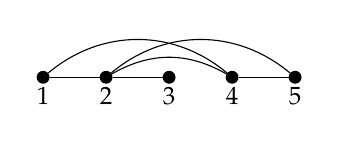
\begin{tikzpicture}[decoration={
          markings,
          mark=at position 0.5 with {\arrow[scale=1.5]{>}}}, scale =.8
        ]
        \foreach \i in {1,2,3,4,5}{
          \node[classic] (a\i) at (\i,0) {};
          \node[below] at (a\i) {\small $\i$};
        }
        \draw (a1) -- (a2) -- (a3) (a4) -- (a5);
        \draw (a2) edge[bend left] (a4);
        \draw (a2) edge[bend left=40] (a5);
        \draw (a1) edge[bend left=40] (a4);
      \end{tikzpicture}
      \caption{The graph $G$}
    \end{subfigure}
    \hfill
    \begin{subfigure}[t]{.65\textwidth}\centering
      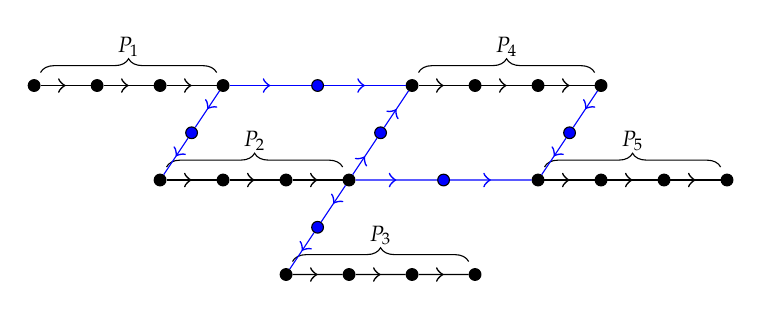
\begin{tikzpicture}[decoration={
          markings,
          mark=at position 0.5 with {\arrow[scale=1.5]{>}}}, scale = .8
        ]

        \foreach \i/\x/\y in {1/0/0,2/2/-1.5,3/4/-3,4/6/0,5/8/-1.5}{
          \foreach \j in {0,...,3}{
            \node[classic] (a\i\j) at ($(\x,\y)+(\j,0)$) {};
          }
          \draw (a\i0) edge[postaction=decorate] (a\i1);
          \draw (a\i1) edge[postaction=decorate] (a\i2);
          \draw (a\i2) edge[postaction=decorate] (a\i3);
          \draw [decorate,decoration={brace,amplitude=5pt,raise=1ex}] (a\i0)
          -- (a\i3) node[midway,yshift=3ex]{\footnotesize $P_\i$};
        }


        \foreach \x/\y in {1/2,2/3,4/5,2/4,1/4,2/5}{          
          \node[classic, fill=blue] (b\x\y) at ($.5*(a\x3) + .5*(a\y0)$) {};
          \draw[blue] (a\x3) edge[postaction=decorate] (b\x\y);
          \draw[blue] (b\x\y) edge[postaction=decorate] (a\y0);
        }          
      \end{tikzpicture}
      \caption{The graph $H$ for $k = 3$ and $s = 4$. The black directed paths
        are the paths $(P_u)_{u \in V(G)}$ and the blue paths are the
        connections $P_{uv}$ of length $s - k +1$ between them.}
    \end{subfigure}
    \caption{An example of our reduction}
  \end{figure}

  Let $C$ be a cycle of $H$ and $u$ the smallest vertex of $G$ such that $C$
  passes by $u^+$ (such vertex exists because $H - \bigcup_{u \in V(G)} u^+$ is
  a forest of subdivided stars with central vertices $(v^-)_{v \in V(G)}$). The
  cycle $C$ alternates at $u^+$ so $H$ is acyclic. Finally, $L^k(H) = G^{\ast
    s}$ has girth $g(s+1) \ge 3(s+1) \ge \ell$, where $g$ is the girth of $G$. 
  
\end{proof}

\section{3-Colouring shift graphs}\label{sec:3COL}
\begin{theorem}\label{thm:3col}
  For any $k\geq 1$, \Col is NP-complete when restricted on the class of $k$-iterated shift graphs (and
  \emph{a fortiori} in shift graphs of odd-girth at least $k$).
\end{theorem}
\begin{proof}
  We design a polynomial time reduction from \Col on general graphs to \Col on $k$-iterated
  shift graphs. For simplicity, we first describe our reduction for shift graphs
  before adapting it to $k$-iterated shift graphs, as the latter case is more technical, but the ideas are essentially identical. We will equivalently view proper colourings
  of $L(\orG)$ as arc-colourings of $\orG$, that is an assignment of colors to $A(G)$
  such that $u\to v$ and $v\to w$ have distinct colors for all $u,v,w \in V(G)$.

\paragraph{The gadget H.}
  We construct an acyclic oriented graph $\orH$ such that $\chi(L(\orH))=3$, having a
  marked vertex $x$ with the following property: in any 3-arc-colouring of $\orH$
  the set of arcs entering $x$ uses exactly two colours. 


\nicolas{I think everything works fine by taking a graph $T$ with
  odd girth $k$ and a minimum number of vertex $n$ and such that
  $\chi(L(T)) = 4$. Then, we don't have to consider higher odd girths
  separatly. The fact that $T$ comes from a tournament is not
  essential. Very little has to be changed in the proof.}

  
  Consider the minimum value of $n\in \mathbb N$ such that the transitive $n$-vertex tournament $\orTn$ satisfies
  $\chi(L(\orTn))=4$. Let $v_{n-1}$ and $v_n$ respectively denote the vertices of $\orTn$ with respective in-degrees
  $n-2$ and $n-1$. % Let $S_n$ be the subgraph of $T_n$
  % obtained by removing all the arcs $uv_n$ with $u \in V(G) \setminus
  % \{v_{n-1},v_n\}$. Given an arc-colouring $\alpha$ of $S_n$,
  % let $\beta$ be the arc-colouring of $T_n$ such that $\beta(xy) = \alpha(xy)$
  % if $xy\in A(S_n)$ and $\beta(uv_n) = \alpha(uv_{n-1})$ for all
  % $u \in V(T_n) \setminus \{v_{n-1},v_n\}$. The arc-colouring $\beta$ is
  % proper because $uv_n$ and $uv_{n-1}$ are twins in $L(T_n)$. Since $\alpha$ and
  % $\beta$ use the same amount of colours and $S_n$ is a subgraph of $T_n$, we
  % have $\chi(L(S_n)) = \chi(L(T_n)) = 4$.
  Let $\orH$ be the graph obtained from $\orTn$ by iteratively removing arcs entering $v_{n-1}$
  until the chromatic number of its line digraph drops to three. Note that
  $\overrightarrow{S_n} := \orTn-\{uv_{n-1} : u \in V(T_{n})\setminus\{v_{n-1},v_{n}\}\}$ is the
  transitive tournament on the vertices $V(T_n)\setminus \{v_{n-1}\}$, with an
  additional vertex $v_{n-1}$ whose only incident arc ends in the sink $v_n$. Thus
  $\orSn$ is 3-arc-colourable,  and $\orH$ is well defined.


  % \nicolas{Typos in the paragraph below: line 5, it should be $\{1,
  %   3\}\setminus c$ and line 7 it should be colour different from 2
  %   and $c$.}

  
  Let $uv_{n-1}$ be the last arc removed in the construction of $\orH$. We thus have
  $\chi(L(\orH + uv_{n-1})) = 4$ and $\chi(L(\orH)) = 3$. Let $\alpha$ be a proper
  3-colouring of $L(\orH)$, where $v_{n-1}v_n$ is without loss of generality
  coloured 1. The arcs entering $v_{n-1}$ cannot use the colour 1, so they use
  at most two colours. Suppose that they are all using the same colour, say
  2 (see \cref{fig: GadgetH}). Let $c := \alpha(uv_n)$ (note that $c$ is well defined as $u\to v_n$ is an arc of $\orH$) and $\beta$ be the 3-colouring of $L(\orH+uv_{n-1})$
  such that $\beta(uv_{n-1}):= c$,
  $\beta(v_{n-1}v_n) \in \{1,3\} \setminus \{c\}$ and $\beta(xy) = \alpha(xy)$
  for all other arcs. The arc-colouring $\beta$ uses three colours like $\alpha$ and we claim that it
  is a proper colouring of $L(\orH+uv_n)$. 
  As $\alpha$ is proper, it suffices to check 
  that the colourings of the arcs $uv_{n-1}$ and $v_{n-1}v_n$ do not create a monochromatic edge. As $v_n$ is a sink, and as $uv_n$ was colored with $c$ by $\alpha$, note that the arc $uv_{n-1}$ cannot have a neighbour of colour $c$ in $L(\orH+uv_n)$.
  Moreover, $v_{n-1}v_n$ is the only arc of $L(\orH+uv_n)$ starting in $v_{n-1}$, and uses a colour different from 2 and $c$, showing that $\beta$ is a proper $3$-colouring. This contradicts 
  $\chi(L(\orH+uv_n))=4$. We thus deduce that the set of arcs entering $v_{n-1}$ in $H$ use both the colours 2 and 3.
  To sum up, $\orH$ is 3-colourable and in each 3-arc-colouring of $\orH$, the arcs
  entering the marked vertex $x:=v_{n-1}$ use two different colours.
  
\begin{figure}[htb]
  \centering  
  \includegraphics[scale=1]{GadgetH}
  \caption{In red, the coloration $\alpha$ depicted in  the first part of the proof of \cref{thm:3col}.}  
  \label{fig: GadgetH}
\end{figure}

  
  
  % We construct an acyclic oriented graph $H$ with two marked arcs $e$ and $f$ with a
  % common marked head $x$ such that any 3-arc-colouring of $H$ colours $e$ and
  % $f$ differently. Let $H$ be the oriented graph on ten vertices $u_0, \ldots, u_8$ and
  % $x$ constructed as follows (see \cref{fig:gadget_3col}). For each
  % $i, j \in \{0, \ldots, 6\} \cup \{8\}$, add the arc $u_i \to u_j$ if
  % $i < j < i+5$ (in black in \cref{fig:gadget_3col}). Add also the arcs
  % $u_3 \to u_7$, $u_4 \to u_7$ and $u_5 \to x$, $u_6 \to x$ (respectively in red
  % and blue in \cref{fig:gadget_3col}). In $H$, $x$ is a
  % sink and a computer check shows that $H$ is 3-arc-colourable, and that all
  % 3-arc-colourings of $H$ use distinct colours on $u_5 \to x$ and $u_6 \to
  % x$ (see \cref{sec:computer_check}).

  % \begin{figure}[h!]
  %   \centering
  %   \begin{tikzpicture}[decoration={
  %       markings,
  %       mark=at position 0.5 with {\arrow[scale=1.5]{>}}}
  %     ]
  %     \foreach \i in {0,...,8}{
  %       \node[classic] (\i) at (\i,0) {};
  %       \node[below left] at (\i) {$u_{\i}$};
  %     }

  %     \node[classic] (x) at (5.5,-1.5) {};
  %     \node[below left] at (x) {$x$};

  %     \foreach \i in {0,...,6}{
  %       \pgfmathsetmacro{\a}{int(\i+1)}
  %       \pgfmathsetmacro{\b}{min(int(\i+4),8)}
  %       \foreach \j in {\a,...,\b}{
  %         \ifthenelse{\j = 7}{}
  %         {\draw (\i) edge[bend left=(\j-1-\i)*20, postaction=decorate] (\j);}
  %       }
  %     }
  %     \foreach \i in {3,4}{
  %       \draw[color1] (\i) edge[bend left=(6-\i)*20, postaction=decorate] (7);
  %     }
  %     \draw[color3,postaction=decorate] (5) -- (x);
  %     \draw[color3,postaction=decorate] (6) -- (x);
  %   \end{tikzpicture}
  %   \caption{The gadget $H$}
  %   \label{fig:gadget_3col}
  % \end{figure}

  \paragraph{Constructing the shift graph.}
  Let $G$ be a graph. We contruct an acyclic oriented graph $\orGp$ such that
  $\chi(G) \le 3$ if and only if $\chi(L(\orGp)) \le 3$ as follows. Fix an arbitrary total order $<$ on the
  vertex set of $G$ and for each vertex $u$ of $G$, take a copy $\orHu$
  of $\orH$, with an arc $e_u:=x_u \to y_u$ starting in the marked vertex $x_u$ of
  $H_u$ and ending in a new pendant vertex $y_u$. For each edge $uv \in E(G)$, with
  $u < v$, add the arc $x_u \to x_v$ (see \cref{fig:NP-col}). The oriented graph
  $\orGp$ constructed is acyclic because each copy $\orHu$ of $\orH$ is acyclic and
  separated from the rest of $G'$ by the cut vertex $x_u$, and the additional
  edges can be ordered acyclically following the order on the vertices of
  $G$. Therefore $L(\orGp)$ is a shift graph. 
  
  We will now show that $G$ is 3-colourable if and only if $L(\orGp)$ is 3-colourable.

  \begin{figure}[h!]
    \begin{subfigure}[t]{.3\textwidth}
      \centering
      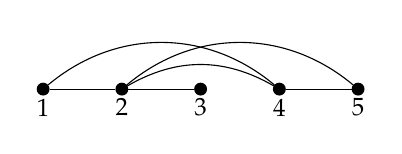
\begin{tikzpicture}
        \foreach \i in {1,2,3,4,5}{
          \node[classic] (a\i) at (\i,0) {};
          \node[below] at (a\i) {\small $\i$};
        }
        \draw (a1) -- (a2) -- (a3) (a4) -- (a5);
        \draw (a2) edge[bend left] (a4);
        \draw (a2) edge[bend left=40] (a5);
        \draw (a1) edge[bend left=40] (a4);
      \end{tikzpicture}
      \caption{A graph $G$}
    \end{subfigure}
    \hfill
    \begin{subfigure}[t]{.65\textwidth}
      \centering
      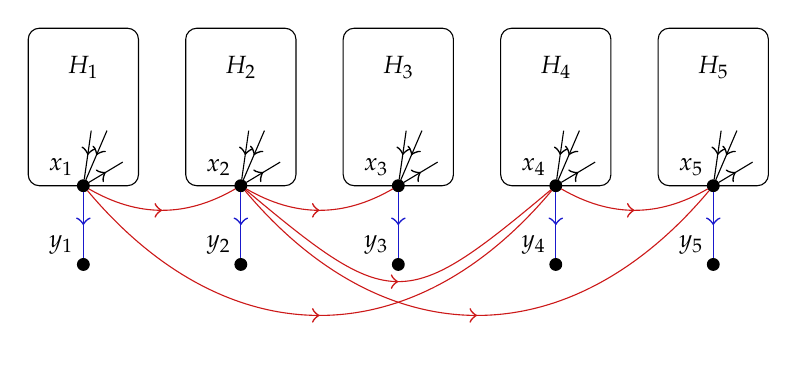
\begin{tikzpicture}[decoration={
        markings,
        mark=at position 0.5 with {\arrow[scale=1.5]{>}}}
      ]
        \foreach \i in {1,2,3,4,5}{
          \begin{scope}[shift={(2*\i,0)}]
            \draw[rounded corners] (-.2,0) rectangle (1.2,2);
            \node[classic] (x\i) at (.5,0) {};
            \node[above left] at (x\i) {\small $x_{\i}$};
            \node[classic] (y\i) at (.5,-1) {};
            \node[above left] at (y\i) {\small $y_{\i}$};
            \node (H\i) at (.5,1.5) {\small $H_{\i}$};
            \draw[postaction=decorate] (.6,.7) -- (x\i);
            \draw[postaction=decorate] (.8,.7) -- (x\i);
            \draw[postaction=decorate] (x\i) -- (1,.3);

            \draw[color3,postaction=decorate] (x\i) -- (y\i);
          \end{scope}
        }

        \draw[color1] (x1) edge[bend right,postaction=decorate] (x2);
        \draw[color1] (x2) edge[bend right,postaction=decorate] (x3);
        \draw[color1] (x4) edge[bend right,postaction=decorate] (x5);
        \draw[color1] (x2) edge[bend right=40,postaction=decorate,looseness=1.6] (x4);
        \draw[color1] (x2) edge[bend right=50,postaction=decorate,looseness=1.2] (x5);
        \draw[color1] (x1) edge[bend right=50,postaction=decorate,looseness=1.2] (x4);

      \end{tikzpicture}
      \caption{The oriented graph $\orGp$ constructed. The blue arcs $x_i \to y_i$
        correspond to the vertices of $G$ and the red arcs to its edges.}
    \end{subfigure}
    \caption{Constructing an equivalent shift graph.}
    \label{fig:NP-col}
  \end{figure}

  \paragraph{Equivalence of the instances.}
  Assume that there exists proper 3-colouring $\alpha$ of $G$. Colour each arc of $\orGp$
  starting in $x_u$ with the colour $\alpha(u)$ of $u$. At this stage it remains
  only to colour the copies of $\orH$. Let $\beta$ be a 3-arc-colouring of $\orH$. For
  each copy $\orHu$, permute the colours of $\beta$ such that the arcs entering
  $x_u$ use the two colours in $[3]$ different from $\alpha(u)$. We claim that the resulting colouring
  is a 3-arc-colouring of $\orGp$. Indeed, at each $x_v$, all the arcs starting in
  $x_v$ have an identical colour $\alpha(v)$, and the arcs entering $x_v$ are
  either coming from the copy $\orHv$ or of the form $x_u \to x_v$ for some
  $u < v$, in both case they use colours different from $\alpha(v)$. Thus
  $L(\orGp)$ is 3-colourable.

  Conversely, in a proper 3-arc-colouring $\beta$ of $\orGp$, observe that by the aforementioned property of $\orH$, for each $u\in V(G)$, the set of arcs entering the marked vertex $x_u$ uses exactly $2$ colors, hence all the
  arcs starting in $x_u$ in $\orGp$ are coloured identically. Colour $u$ with this
  colour for each $u\in V(G)$. We claim that this gives a proper 3-colouring that we denote with $\alpha$. Indeed, given any edge $uv$ in $E(G)$ with $u<v$, the colour of $u \in V(G)$ with respect to $\alpha$
  is the colour of $x_u\to x_v$ with respect to $\beta$, which must differ from the colour of $x_v \to y_v$ with respect to $\beta$. In particular, note that the colour of $x_v\to y_v$ with respect to $\beta$ is the colour of $v \in V(G)$ with respect to $\alpha$. Thus $G$ is 3-colourable.

  \todo[inline]{the proof is broken for $k$-iterated shift graph.}
  \paragraph{$k$-iterated shift graphs.}
  We fix $k\geq 1$.
  To adapt our reduction to $k$-iterated shift graph, we will first need to
  change our gadget. Given a $k$-iterated line digraph $\orGd$ of an oriented
  acyclic graph $\orGu$, we will for convenience see the $k$-colourings of $\orGd$ as
  $k$-colourings of the $k$-paths of $\orGu$ such that the every two $k$-paths of the form $u_0\dots u_k$ and $u_1\dots u_{k+1}$ are coloured differently.

  For our gadget, we construct an acyclic oriented graph $\orH$ such that
  $\chi(L^k(\orH))=3$, with a marked $(k-1)$-path $X$ with the following property:
  in any 3-colouring of $L^k(\orH)$, the set of $k$-paths with suffix $X$ uses
  exactly two colours.

  Consider the minimum value of $n\in \mathbb N$ such that the vertex transitive tournament $\orTn$ verifies
  $\chi(L^k(\orTn))=4$. For each $i \in [n]$, let $v_i$ be the (unique) vertex of in-degree
  $i-1$ in $\orTn$. % Let $S_n$ be the subgraph of $T_n$ obtained by removing all
  % the arcs $v_jv_{n-i}$  for all $i \in \{0, \dots, k-1\}$ and 
  % $j<n-i-1$. The oriented graph $S_n$ consists of a transitive tournament on the
  % vertices $\{v_i : i \in [n-k]\}$, with a $k$-path on the vertices
  % $v_{n-k}, \dots v_n$. Let $\phi$ be the following map from the $k$-paths of if
  % $xy\in A(S_n)$ and $\beta(uv_n) = \alpha(uv_{n-1})$ for all
  % $u \in V(T_n) \setminus \{v_{n-1},v_n\}$. The arc-colouring $\beta$ is proper
  % because $uv_n$ and $uv_{n-1}$ are twins in $L(T_n)$.  $T_n$ to the $k$-paths
  % of $S_n$. For all $k$-paths $P$ of $S_n$, $\phi(P) = P$. Any other $k$-path
  % $P$ of $T_n$ is the concatenation of a $i$-path $Q$ on the vertices of
  % $\{v_j : j < n-k\}$ and a $k-i-1$-path on vertices of
  % $\{v_j: \in \{n-k, \dots n\}$. For such paths, $\phi(P)$ is the concatenation
  % of $Q$ with $v_{n-k}, \dots v_{n-k+i-1}$. In particular, note that $P$ and
  % $P'$ are consecutive in $T_n$, \emph{i.e.} the suffix of length $k-1$ of $P$
  % is the prefix of length $k-1$ of $P'$, then $\phi(P)$ and $\phi(P')$ are
  % consecutive in $S_n$. Thus, given a colouring $\alpha$ of $L^k(S_n)$, the
  % colouring $\beta$ of $L^k(T_n)$ such that $\beta(P) = \alpha(\phi(P))$ for all
  % $P$ is a proper colouring. Since $\alpha$ and $\beta$ use the same amount of
  % colours and $S_n$ is a subgraph of $T_n$, we have
  % $\chi(L(S_n)) = \chi(L(T_n)) = 4$.
  Let $\orH$ be the subdigraph of $\orTn$ obtained by removing iteratively arcs of the form
  $v_iv_{n-k}$ with $i<n-k$ until the chromatic number of its $k$-iterated line
  digraph drops to three. Note that $\orSn:= \orTn-\{v_iv_{n-k} : i <n-k\}$ is the
  transitive tournament on the vertices
  $v_1, \ldots, v_{n-k-1}, v_{n-k+1}, \ldots, v_n$ with the additional vertex
  $v_{n-k}$ and all arcs of the form $v_{n-k}v_j$ with $j>n-k$. As such,
  $L^k(\orSn)$ is isomorphic to the $k$-iterated line digraph of the transitive
  tournament on $n-1$ vertices, with one additional isolated vertex, 
  corresponding to the $k$-path $v_{n-k} \ldots v_n$. So $L^k(\orSn) = 3$ and $\orH$
  is well defined. Let $uv_{n-k}$ be the last arc removed in the construction
  of $\orH$. We then have $\chi(L^k(\orH))= 3$ and $\chi(L^k(\orH+uv_{n-k}))=4$.

  Let $\alpha$ be a 3-colouring of $L^k(\orH)$, and without loss of generality
  assume that the $k$-path $v_{n-k} \dots v_n$ is coloured 1 by $\alpha$. We
  will now argue that the set of $k$-paths with suffix $X:=v_{n-k}\dots v_{n-1}$
  uses both the colours 2 and 3.
%   , and thus that all the $k$-paths with
%   prefix $X$ in the second part of the reduction are coloured 1. 
  First, since
  $P:=v_{n-k}\dots v_n$ is coloured 1 and is the only $k$-path starting in
  $v_{n-k}$, the $k$-paths of $\orH$ with suffix $X$ all have their colours in
  $\{2,3\}$.


  Suppose for a contradiction that they all use the same colour, say 2. In the next paragraph, we let $P_0:=v_{n-k}\dots v_n$. Let $c$ be the colour of
  the $k$-path $uv_{n-k+1} \dots v_n$. Let $f$ be the map from the
  $k$-paths of $\orH+uv_{n-k}$ to the $k$-paths of $\orH$ defined as follows. For each $k$-path $P$
  avoiding the arc $uv_{n-k}$, we let $f(P) =P$. Given a $k$-path $P$ using
  $uv_{n-k}$, let $Q$ denote its prefix ending at $u$ and $R$ its suffix starting
  at $v_{n-k}$ and let $f(P)$ be the concatenation of $Q$ and
  $u v_{n-k+1} \dots v_{n-k+1+q}$ where $q$ is the length of $Q$. Observe that for every 
  two $k$-paths $P,P'$ in $\orH+uv_{n-k}$ distinct from $P_0$, if $P\to P'$ in $L^k(\orH+uv_{n-k})$, then we also have $f(P)\to f(P')$ in $L^k(\orH)$. In more sophisticated terms, $f$ induces a digraph homomorphism from $L^k((\orH+uv_{n-k})-P_0)$ to $L^k(\orH)$.
%   In particular,
%   if $P$ and $P'$ are consecutive in $T_n$, then so are $f(P)$ and
%   $f(P')$. 
  Let $\beta$ be the 3-colouring of $L(\orH+uv_{n-k})$ defined as
  follows. 
  \begin{enumerate}
  \item\label{item: k-gadget-1} For any $k$-path $P$ of $\orH+uv_{n-k}$ without $X$ as a suffix or prefix, we let
  $\beta(P) := \alpha(f(P))$.
  \item\label{item: k-gadget-2} For any $k$-path $P$ of $\orH+uv_{n-k}$ having $X$ as a suffix, 
  \begin{enumerate}
   \item\label{item: k-gadget-2a} either $P$ is a $k$-path of $\orH$ and we set $\beta(P):=\alpha(P)=\alpha(f(P))=2$,
   \item\label{item: k-gadget-2b} or $P=uv_{n-k}\dots v_{n-1}$ and we set $\beta(P) := \alpha(f(P))=
   \alpha(uv_{n-k+1}\dots v_n) = c$.
  \end{enumerate}
  \item\label{item: k-gadget-2} For $P=P_0$ (which is the only $k$-path of $\orH+uv_{n-k}$ having $X$ as a prefix), we let $\beta(P)$ be any colour from $\{1,3\}\setminus \{c\}$.
  \end{enumerate}
  We show that $\beta$ is a 3-colouring of $L^k(\orH+uv_{n-k})$. First, observe that by our previous remark, for every two paths $P,P'$ distinct of $P_0$ from $\orH+uv_{n-k}$, as 
  $f(P)$ and $f(P')$ are adjacent in $L^k(\orH)$, we have $\beta(P)=\alpha(f(P))\neq\alpha(f(P'))=\beta(P')$.  
  This implies that the only arcs of $L^k(\orH+uv_{n-k})$ for which it remains to check that $\beta$ does not colour them monochromaticaly are the ones incident to $P_0$. In particular, note that every such arc is of the form $P\to P_0$, for some path $P$ of type \cref{item: k-gadget-2}. If $P$ has type \cref{item: k-gadget-2a}, then we have $\beta(P)=2$, while $\beta(P_0)\neq 2$ by construction. If $P$ has type \cref{item: k-gadget-2b}, then $\beta(P)=c$ and again by construction $c\neq \beta(P_0)$. It thus implies that $\beta$ is indeed a proper 3-colouring of $L^k(\orH+uv_{n-k})$. However, this contradicts our previous observation that $\chi(L^k(\orH+uv_{n-k}))=4$. We thus conclude that every 3-colouring of $L^k(\orH)$ gives to the set of $k$-paths having  $X$ as a suffix exactly two colors.
  
%   Any $k$-path $P$ with suffix $X$ in
%   $\orH+uv_{n-k}$ is either a $k$-path of $H$, in which case $\alpha(P)=2$ and we
%   define $\beta(P) = 2$, or the $k$-path $uv_{n-k}\dots v_{n-1}$, in which
%   case we let $\beta(P) = \alpha(uv_{n-k+1}\dots v_n) = c$. The only remaining
%   $k$-path where $\beta$ is undefined is the path $P = v_{n-k} \dots v_n$ with
%   $X$ as prefix. 
%   By construction all its incident paths in $L^k(\orH+uv_{n-k})$ are
%   colored 2 and $c$ by $\beta$, so we can colour this path with a colour from
%   $\{1,3\}\setminus\{c\}$. The colouring $\beta$ is a proper 3-colouring of
%   $L^k(\orH+uv_n)$, which contradicts $\chi(L^k(\orH+uv_{n-k}))=4$. So the set of $k$-paths of $\orH$ with suffix $X=v_{n-k}\dots v_{n-1}$ uses both the colours 2 and 3 in $\alpha$. To
%   sum up, $L^k(\orH)$ is 3-colourable and in each 3-colouring of $L^k(\orH)$, the
%   $k$-paths with prefix $X$ use two different colours.

  We now finish the reduction in a similar way as for shift graphs. Let $G$ be a
  graph, with an arbitrary order on its vertices. We define an oriented graph $\orGp$ as follows. For each vertex $u$ of $v$,
  take a copy $\orHu$ of $\orH$ and a new pendant vertex $y_u$, and attach an arc $x_uy_u$ to
  the last vertex $x_u$ of the marked $(k-1)$-path $X_u$ of $\orHu$. For each edge
  $uv$ of $G$ with $u<v$, we add a pending arc $x_uz_{uv}$ to $x_u$ and identify
  the marked $(k-1)$-path $X_v$ with the $(k-1)$-path formed by concatenating
  the $(k-2)$-suffix of $X_u$ with $x_uz_{uv}$. \ugo{I'm afraid that $\orGp$ is not always well-defined... Unless I missed smg.} As a result, we have an arc $X_ux_v\to X_vy_v$
  in $L^k(\orGp)$.
%   the $k$-paths
%   $X_ux_v$ and $X_vy_v$ are consecutive.  
  The oriented graph $\orGp$ constructed is
  acyclic because each copy $\orHu$ is acyclic, and the vertex set of $\orGp$ can be ordered following the
  order of the vertices of $G$. In such an order for every vertices $u<v$ of $G$, every arc of $\orGp$ between disjoint subgraphs $\orHu$ and $\orHv$ has its tail in $\orHu$ and its head in $\orHv$. It follows that $\orGp$ is indeed acyclic.
  We consider the subgraph $L$ of $L^k(G')$
  induced by the $k$-paths that contain at most one arc between different
  vertices labelled $x_u$ for some $u$.

  We will show that $L$ is 3-colourable if and only if $G$ is 3-colourable. 
  
  \paragraph{Equivalence of the instances for $k$-iterated shift graphs.}
  We first assume that $G$ is 3-colourable and let
  $\alpha$ be a proper 3-colouring of $G$. Let $\beta$ be the 3-colouring of $L$
  defined as follows. First, for each $u \in V(G)$, colour each $k$-path of $G'$
  with penultimate vertex equal to $x_u$ with the colour $\alpha(u)$. Each
  remaining $k$-path of $L$ is fully contained in some $H_u$ for some $u$
  because we removed from $L$ the $k$-paths containing more than one arc between
  different vertices labelled $x_u$ for some $u$. For each $u$, all the
  $k$-paths with suffix $X_u$ of $H_u$ are identically coloured, so one can
  permute the colours in a fixed 3-colouring of $L^k(H)$ to colour
  $L^k(H_u)$. Two consecutive $k$-paths of $L$ are either both contained in some
  $H_u$, or with suffix and prefix equal to some $X_u$, or with prefix equal to
  some $X_u$ and formed by the $(k-2)$-suffix of $X_u$ concatenated with
  $x_vy_v$ for some $v>u$ with $uv \in E(G)$. In either case, their colours are
  different by construction. Conversely, given a proper 3-colouring $\beta$ of
  $L$, let $\alpha$ be the colouring of $G$ such that for each $u$, $\alpha(u)$
  is the colour in $\beta$ of the $k$-path with prefix $X_u$ finishing in
  $y_u$. By design of $H$, all $k$-path with prefix $X_u$ are identically
  coloured and so $\alpha(u)$ and $\alpha(v)$ are different for each
  $uv \in E(G)$ with $u<v$, because the paths $X_ux_v$ and $X_vy_v$ are
  consecutive by construction and
  $\alpha(u) = \beta(X_ux_v) \neq \beta(X_vy_v) = \beta(v)$.
\end{proof}

In the next proof, an \emph{in-forest} (resp.\ \emph{out-forest}) is an oriented forest in which each vertex has in-degree (resp.\ out-degree) at most $1$. Observe that in particular, every component of an in-forest (resp.\ out-forest) has exactly one vertex with in-degree (resp. out-degree) equal to 0, which we call the \emph{root} of its component.

We now prove that if one restricts to shift graphs of large girth (and not large
odd-girth as in \cref{thm:3col}), 3-colouring becomes a trivial problem.
\begin{proposition}
  All shift graphs of girth at least five are 3-colourable.
\end{proposition}
\begin{proof}
  Let $G$ be a shift graph of girth at least five and denote $\orG$ its shift
  orientation. Let $\orH$ be an oriented acyclic graph which is a root digraph
  of $\orG$. We will identify $V(G)$ with $A(\orH)$. Observe that each vertex of
  $\orH$ has either in-degree or out-degree at most one, as a vertex with both
  in- and out-degree at least two would produce a four-cycle in the line
  digraph. We partition the vertices of $\orH$ in two subsets: let $X$ be the
  set of vertices of $\orH$ with in-degree at most one, and $Y:=V(H)\setminus X$
  be the remaining vertices, which all have out-degree at most one. We now
  partition the arcs of $\orH$ in four subsets. We let $A_X$ and $A_Y$
  respectively denote the sets of arcs having both extremities in $X$ and $Y$
  respectively. We let $A_{X\to Y}$ (resp.\ $A_{Y\to X}$) denote the set of arcs
  of $\orH$ having their tail in $X$ (resp.\ $Y$) and their head in $Y$ (resp.\
  $X$).  Note that $A_{X\to Y}$ and $A_{X\to Y}$ both form independent sets in
  $G$. We color all vertices of $A_{X\to Y}$ with one colour, say 1.
  
  We now show that the arcs of $A_X\cup A_Y \cup A_{Y\to X}$ form a forest in
  $G$, and therefore can be coloured with two additional colours, which results
  in a proper 3-arc-colouring of $\orH$.  First, observe that as $X$ does not
  contain vertices with in-degree $2$, $\orH[X]=(X,A_X)$ must be an
  out-forest. Symmetrically, $\orH[Y]=(Y,A_Y)$ is an in-forest. Observe also
  that the arcs of $A_{Y\to X}$ must form a matching, and can only connect a
  root of some component of $\orH[Y]$ to a root of some component of
  $\orH[X]$. It follows that the induced subgraph
  $G[A_X\cup A_Y\cup A_{Y\to X}]$ is a forest. More precisely, one can observe
  this graph is isomorphic to the graph obtained when contracting each edge of
  the matching $A_{Y\to X}$, and when removing all roots of those components of
  $\orH[X]$ and $\orH[Y]$ which are not incident to some arc in $A_{Y\to X}$.
\end{proof}
\section{Recognising shift graphs}\label{sec:recognition}

% By Schaefer's dichotomy theorem~\cite{schaefer1978Complexity}, the following
% problem is NP-complete.
Recall that a $3$-CNF formula is a boolean formula $\varphi$ in conjonctive normal form (CNF), in which each clause contains 3 litterals. Such a formula $\varphi$ is called \emph{monotone} if all variables always appear positively, i.e.\ no litteral has the form $\neg x$ for some variable $x$.  
Lov\'asz \cite{lovasz1973Covering} proved that the following problem is NP-complete.

\begin{csproblem}{Monotone Not all equal 3-SAT (MNAE-3SAT)}
  Given as input a monotone 3-CNF formula $\phi$, decide if there exists a valuation of
  the variables such that each clause of $\phi$ contains both variables set ot true and false.
\end{csproblem}

Note that \MNAE is equivalent to the problem of deciding whether a given $3$-regular hypergraph is $2$-colourable. In particular, this hypergraph formulation was the one used in \cite{lovasz1973Covering}. In order to prove the next result, we will design a polynomial time reduction to $\MNAE$, inspired by the one from \cite{chvatal1990Note}.

\begin{theorem}
  For each $k \ge 1$, the problem of recognising whether a graph is a $k$-iterated shift graph (or equivalently, the
  support of the $k$-iterated line digraph of
  an acyclic oriented graph) is NP-complete.
\end{theorem}


\begin{proof}
  % Here again, we first explain the reduction to shift graphs before adapting it
  % to iterated shift graphs.
  Let $k \in \mathbb{N}$. We reduce \MNAE to the problem of recognising a $k$-iterated shift
  graph. Let $\phi$ be a monotone 3-CNF formula with $m$
  clauses and $n$ variables. We construct a graph $G_\phi$ of size $O(mnk)$ which is a $k$-iterated shift graph if
  $\phi$ is a valid instance of \textsc{MNAE-3SAT}, but is not a shift graph (and
  \emph{a fortiori} not a $k$-iterated shift graph) if $\phi$ is not a valid
  instance of \textsc{MNAE-3SAT}. 

  \paragraph{Gadgets.}
  We first describe a gadget that will be used later for encoding the
  variables. Let $H$ be the 4-sun, that is the graph on eight vertices composed
  of a 4-cycle with one pendant edge attached to each of the vertices on the
  cycle. For each variable $x$, consider the gadget composed of a path $U_x$ on
  $8m+1$ vertices. Denote $u_x^0, \dots u_x^{4m-1}$ every other vertex of $U_x$,
  starting from the second vertex of $U_x$. For each $i \in \{0, \dots, 4m-1\}$
  we connect $u_x^{i}$ to the first vertex of the jaw of a comb $Q_i$ of length
  $k+1$. Denote $v_x^{i}$ the last vertex of the jaw of this comb and
  $w_x^{i}$ the vertex adjacent to $v_x^{i}$ via the last tooth.%  \ugo{Why not
    % simply call them $v_x^i$ and $w_x^i$?}
  Connect each $u_x^{i}$ to a
  distinct copy $H_x^i$ of $H$ via one of its vertices of degree three that we
  will call $t_x^{i}$ (see \cref{fig:variable_gadget}). For each variable $x$,
  let $L_x$ denote a disjoint copy of this graph, and let $M_x$ be the subgraph
  of $L_x$ obtained by removing all vertices of the graphs $H_x^i$, except the
  vertices $(t_x^{i})_{0 \le i \le 4m-1}$. In particular, $M_x$ is connected and contains
  $\bigcup_{i=0}^{4m-1} \{t_x^{i}, v_x^{i}, w_x^{i}\} \cup V(U_x)$.


  \begin{figure}[h!]
    \centering
    \begin{tikzpicture}[scale = 1.5]
      \foreach \i in {0,...,3}{
        \begin{scope}[shift={(2*\i,0)}]
          \coordinate (a\i) at (0,0);
          
          \foreach \j in {1,...,3}{
            \node[classic,fill=red] (e\i\j) at (0,-.75*\j) {};
            \node[classic,fill=red] (d\i\j) at (-1.,-.75*\j) {};
            \draw (d\i\j) -- (e\i\j);
          }

          \foreach \j in {1,2}{
            \pgfmathsetmacro{\jj}{int(\j+1)}
            \draw (e\i\j) -- (e\i\jj);
          }

          \node[classic,fill=red] (H\i11) at (0,.5) {};
          \node[classic] (H\i12) at (-.25,.25) {};
          \node[classic] (H\i21) at (.25,.75) {};
          \node[classic] (H\i22) at (.5,.75) {};
          \node[classic] (H\i31) at (0,1) {};
          \node[classic] (H\i32) at (0,1.25) {};
          \node[classic] (H\i41) at (-.25,.75) {};
          \node[classic] (H\i42) at (-.5,.75) {};
          \draw (H\i11) -- (H\i21) -- (H\i31) -- (H\i41) -- (H\i11);
          \draw (H\i11) -- (a\i) -- (e\i1);
          \foreach \j in {1,...,4}{
            \draw (H\i\j1) -- (H\i\j2);
          }
          
        \end{scope}        
        
      }


      \node[classic,fill=red] (b) at (-1,0) {};

      \draw (b) -- (a0);

      \foreach \i in {0,...,3}{
        \coordinate (b\i) at (2*\i+1,0);
        \pgfmathsetmacro{\j}{\i+1}
        \draw (a\i) -- (b\i) -- (a\j);
      }

      \foreach \i in {0,...,3}{

        \node[classic,fill=red] at (a\i) {};
        \node[classic,fill=red] at (b\i) {};
      }
      
      
      \node[below right=-.15cm] at (H011) {\footnotesize $t_x^0$};
      \node[below right=-.15cm] at (a0) {\footnotesize $u_x^0$};
      \node[below left=-.1cm] at (e03) {\footnotesize $v_x^0$};
      \node[below left=-.1cm] at (d03) {\footnotesize $w_x^0$};
      \node[below right=-.15cm] at (H111) {\footnotesize $t_x^1$};
      \node[below right=-.15cm] at (a1) {\footnotesize $u_x^1$};
      % \node[below right=-.15cm] at (b0) {\footnotesize $u_x^1$};
      \node[below left=-.1cm] at (e13) {\footnotesize $v_x^1$};
      \node[below left=-.1cm] at (d13) {\footnotesize $w_x^1$};
      \node[below right=-.15cm] at (H311) {\footnotesize $t_x^{4m-1}$};
      \node[below right=-.15cm] at (a3) {\footnotesize $u_x^{4m-1}$};
      \node[below left=-.1cm] at (e33) {\footnotesize $v_x^{4m-1}$};
      \node[below left=-.1cm] at (d33) {\footnotesize $w_x^{4m-1}$};

      \draw [decorate,decoration={brace,amplitude=5pt,mirror,raise=1ex}] (e33)
      -- (e31) node[midway,xshift=4ex]{\footnotesize $k+1$};

    \end{tikzpicture}  
    \caption{The variable gadget $L_x$. The red vertices induce the subgraph $M_x$.}
    \label{fig:variable_gadget}    
  \end{figure}
  
  For each $i \in \{0,\dots, m-1\}$, if $x,y,z$ denote the three variables
  appearing in the $i$\textsuperscript{th} clause of $\phi$, we attach the
  gadgets $L_x$, $L_y$ and $L_z$ as follows. Add three edges to form a path
  $a_ib_ic_id_i$, where $a_i=w_x^{4i}$, $b_i=w_y^{4i+1}$, $c_i=w_y^{4i+3}$ and
  $d_i=w_z^{4i}$, so that the vertex set
  $\{w_x^{4i}, w_y^{4i+1}, w_y^{4i+3}, w_z^{4i}, v_x^{4i}, v_y^{4i+1},
  v_y^{4i+3}, v_z^{4i}\}$ forms a comb $C_i$ of length three, with jaw
  $w^{4i}_xw_y^{4i+1}w_y^{4i+3}w_z^{4i}$. Denote $G_\phi$ the constructed graph.

  \paragraph{Valid orientations of $G_\phi$.}
  We call an orientation of a graph \emph{valid} if 
  it is a line
  digraph of an acyclic oriented graph. In other words, valid orientations are exactly the acyclic orientations satisfying the two conditions of \cref{lem:line-graph}.
  Before proving that there is a valuation such that
  $\phi$ is a positive instance of $\MNAE$
%   has both variables set to true and false in each clause 
  if and only if $G_\phi$
  admits a valid orientation, we prove several lemmas describing valid
  orientations of $G_\phi$ and some of its subgraphs.

  \begin{claim}\label{cl:sun_orientation}
    Up to isomorphism, there are only two valid orientations of the 4-sun, which are opposite from each other (see
    ~\cref{fig:sun_orientation}). In these orientations, the 4-cycle is
    alternating and all vertices of degree three are transitive.
  \end{claim}
  \begin{figure}[ht]
    \centering
    \begin{tikzpicture}[decoration={
        markings,
        mark=at position 0.5 with {\arrow[scale=1.5]{>}}}
      ]
      
      \node[classic] (a) at (0,0) {};
      \node[classic] (a') at (-1,0) {};
      \node[classic] (b) at (1,1) {};
      \node[classic] (b') at (1,2) {};
      \node[classic] (c) at (2,0) {};
      \node[classic] (c') at (3,0) {};
      \node[classic] (d) at (1,-1) {};
      \node[classic] (d') at (1,-2) {};

      \draw[postaction={decorate}] (a) -- (b);
      \draw[postaction={decorate}] (c) -- (b);
      \draw[postaction={decorate}] (a) -- (d);
      \draw[postaction={decorate}] (c) -- (d);

      \draw[postaction={decorate}] (a') -- (a);
      \draw[postaction={decorate}] (b) -- (b');
      \draw[postaction={decorate}] (c') -- (c);
      \draw[postaction={decorate}] (d) -- (d');

    \end{tikzpicture}
    \caption{The only valid orientation of the 4-sun (and its opposite).}
    \label{fig:sun_orientation}
  \end{figure}
  \begin{poc}
    Consider $\orH$ a valid orientation of $H$. Recall that by~\cref{lem:valid},
    the 4-cycles are alternating at each vertex in a shift orientation of shift graph. \ugo{I do not think that it is enough... I suggest the next arguments (in red).
    
    As $\orH$ is acyclic, the 4-cycle $C$ of $H$ contains at least one sink and one source (with respect to the induced orientation on the cycle). Moreover, note that every such orientation $\overrightarrow{C}$ of $C$ containing one transitive vertex contradicts either of the two conditions from \cref{lem:valid}. It implies that the orientation of $C$ induced by $\orH$ is the alternating orientation depicted in \cref{fig:sun_orientation}.} 

  \clement{We wrote below \cref{lem:valid} that it implies that 4 cycles are
    alternating in shift graphs}
  
    Now let $v$ be a vertex of degree
    three in $H$. Without loss of generality, assume that $v$ has no in-neighbour in
    $C$, i.e.\ that it is a source of $C$. Let $u$ be the unique neighbour of $v$ which is not on $C$, and $w$ and $x$ be two
    vertices of $C$ such that $w$ is adjacent to $v$, while $x$ is not. As the orientation of $C$ in $\orH$ alternates, we must have $v\to w$ and $w\to x$ in $\orH$. In particular, the first condition of~\cref{lem:forbidden_config}, then implies that we have $u\to v$ in $\orH$, hence $v$ is transitive. As this reasoning is independent of the choice of $v$ on $C$, we deduce that $\orH$ has the desired form.
  \end{poc}


  \begin{claim}\label{cl:gadget_orientation}
    Consider a valid orientation of $L_x$ for some fixed variable $x$. Then there are only two possible
    orientations for its restriction to $M_x$, which are opposite from each other, and such that
    \begin{itemize}
     \item if $w_x^0 \to v_x^0$ then for all $i$, we have $w_x^{i} \to v_x^{i}$ if $i$
    is even and $v_x^{i} \to w_x^{i}$ if $i$ is odd,
    \item if $v_x^0 \to w_x^0$ then for all $i$, we have $v_x^{i} \to w_x^{i}$ if $i$
    is even and $w_x^{i} \to v_x^{i}$ if $i$ is odd.
    \end{itemize}
  \end{claim}
  \begin{poc}
    Fix a valid orientation $\orLx$ of $L_x$ and without loss of generality, assume that $w_x^0 \to v_x^0$ in $\orLx$, the other case being symmetric.
    For each $i\in \{0,\ldots,4m-1\}$, we let $\orHxi$ denotes the orientation of the subgraph $H_x^i$ induced by $\orLx$.
    By~\cref{cl:sun_orientation}, in each $\orHxi$ all the vertices of degree three are transitive (however,
    each subgraph $H_x^i$ may be oriented in any of its two opposite
    orientations independently of any other copy).

    We first show that for each $i\in \{0,\ldots,4m-1\}$, we have the following
    \begin{enumerate}
    \item\label{item:sink} if $u^{i}_x \to t^{i}_x$ in $\orLx$, then $u^{i}_x$
      is a sink in $\orLx-t_x^{i}$.
    \item\label{item:source} if $t^{i}_x \to u^{i}_x$ in $\orLx$, then $u^{i}_x$
      is a source in $\orLx-t_x^{i}$,
    \end{enumerate}
    We only show \ref{item:sink}, as \ref{item:source} is symmetric. Let
    $i \in \{0,\ldots,4m-1\}$ and assume that $u^{i}_x \to t^{i}_x$ in
    $\orLx$. By \cref{cl:sun_orientation}, $t^{i}_x$ is transitive in $\orHxi$,
    and thus has an in-neighbour in $\orLx$ distinct from $u_x^{2i}$. In
    particular, note that the first condition of \cref{lem:forbidden_config}
    then implies that $u^{2i}_x$ cannot have an out-neighbour in
    $\orLx-t^{2i}_x$, showing \ref{item:source}.
    
    Using once again the first condition of \cref{lem:forbidden_config}, observe
    that the vertices of degree two in $U_x \setminus \{u_0, \dots, u_{4m-1}\}$
    are transitive and that the vertices $u^{i}$ are alternatively sources or
    sinks in $\orLx - \bigcup_it^i_x$. In order to conclude the proof of the
    claim, observe that for $i$ such that $u^i_x$ is a sink in $\orLx - t^i_x$
    (respectively a source), applying iteratively the first condition of
    \cref{lem:forbidden_config} implies that the jaw of the comb $Q_i$ is
    oriented towards $u^i_x$ and each teeth $st$ where $s$ belongs to the jaw is
    oriented $t \to s$ in $\orLx$ (resp. away from $u^i_x$ and $s \to t$). So
    for each $i$, $u^i_x$ is a sink if and only if $w^i_x \to v^i_x$.  In
    particular, because the edge $w^0_xv^0_x$ is oriented $w^0_x \to v^0_x$ and
    the vertices $u^i_x$ are alternatively sources and sinks in
    $\orLx - \bigcup_it^i_x$, this proves that we have $w^i_x \to v^i_x$ for all
    even $i$ and $v^i_x \to w^i_x$ for all odd $i$.



    \clement{The end of the previous proof was false, I changed it.}
    % In particular, as we
    % assumed $w_x^0\to v_x^0$, this implies that for each
    % $i\in \{0,\ldots, 4m-1\}$, if $i$ is even, then $u_x^{2i}$ satisfies
    % \ref{item:sink}, while if $i$ is odd, then $u_x^{2i}$ satisfies
    % \ref{item:source}.
    
    % (if $u^{2i}_x \to t^{2i}_x$ reverse all the orientations in the following
    % reasoning). By \cref{cl:sun_orientation}, $t^{2i}_x$ is transitive in the
    % copy of the 4-sun it belongs to, so $t^{2i}_x$ has an out-neighbour.
    % Therefore, $u^{2i+1}_x$, $u^{2i-1}_x$ and $v^{2i}_x$ are all
    % out-neighbours of $u^{2i}_x$, which proves that $u^{2i}_x$ is transitive.
    % By propagating the same reasoning along the vertices of the jaw of the comb
    % attached to $u^{i}_x$, the jaw of the comb is oriented away from $u^{2i}x$
    % and its teeth away from the jaw. In particular, we have
    % $v^{i}_x \to w^{2i}_x$. We obtain $u^{2i+1}_x \to u^{2i+2}_x$ likewise. The
    % result follows from a straightforward induction on $i$.
  \end{poc}
  
  For each $i\in \{0,\ldots,4m-1\}$, and every orientation $\orCi$ of the comb $C_i$, we say that a teeth $e$ of is 
  \begin{itemize}
  \item \emph{positive} if $e$ is a molar and is oriented away from the jaw, or
    if $e$ is an incisor and is oriented towards the jaw.
   \item \emph{negative} if $e$ is a molar and is oriented towards the jaw, or
     if $e$ is an incisor and is oriented away from the jaw.
  \end{itemize}
  
%   Given a valid orientation of the comb $C_i$, we say that $e_1$ and
%   $e_4$ (respectively $e_2$ and $e_3$) are \emph{positive} if they are oriented
%   away (resp. towards) the jaw, and that they are \emph{negative} otherwise.
  
  \begin{claim}\label{cl:clause_orientation}
    For each $i\in \{0,\ldots,4m-1\}$, in any valid orientation of $C_i$, the teeth of $C_i$ cannot be all positive, or
    all negative. 
    Conversely, any orientation of the teeth of $C_i$ in which the incisors are both positive (resp.\ both negative), and in which at least one molar is
    negative (resp.\ positive) can be extended to a 
    valid orientation of $C_i$ in which the jaw of $C_i$ is a directed path.
  \end{claim}
  \begin{poc}
    We let $a=a_1a_2, \dots,d=d_1d_2$ denote the four teeth of $C_i$ with jaw
    $(a_1,b_1,c_1,d_1)$. Assume towards a contradiction that there exists a
    valid orientation $\orCi$ of $C_i$ making all teeth positive. That is, the
    molars $a$ and $d$ are oriented away from $a_1$ and $d_1$, while
    the incisors $b$ and $c$ are oriented towards $b_1$ and
    $c_1$. Without loss of generality, assume that $b_1 \to c_1$. By
    \cref{lem:forbidden_config}, as $c_1$ has both an in-neighbour and an
    out-neighbour, the edge $a_1b_1$ must be oriented $a_1 \to b_1$ (see \cref{fig:
      proof_3comb}). We then obtain a contradiction as the orientation of the
    induced path $a_2a_1b_1b_2$ contradicts the first condition of
    \cref{lem:forbidden_config}.
%     
%     Hence
%     $b$ has also an in-neighbour and an out-neighbour and $e_1$ is oriented
%     towards $a$, that is $e_1$ is negative. By the symmetry, if we had
%     $c \to b$, $e_4$ would be negative. So $e_1$ or $e_4$ is negative, a
%     contradiction. We claim that symmetric arguments apply to show that there exists no valid orientation of $N$ with all
%     edges $e_j$ negative.

   \begin{figure}[htb]
   \centering  
   \includegraphics[scale=1]{3comb}
   \caption{The orientation depicted in the first part of the proof of \cref{cl:clause_orientation}.}  
   \label{fig: proof_3comb}
   \end{figure}
    
    Conversely, consider an orientation of the teeth $a, \ldots, d$, such that $b$
    and $c$ are say positive, but not all four edges are positive. Say without
    loss of generality $a$ is negative. Then, no matter which orientation $d$ has, orienting the jaw of $C_i$ as a
    directed path from $a_1$ to $d_1$ (as depicted on \cref{fig:variable_gadget})
    gives an orientation of $C_i$ avoiding the forbidden configurations of
    \cref{lem:forbidden_config}, and thus which is valid.
    \begin{figure}[h!]
      \centering
      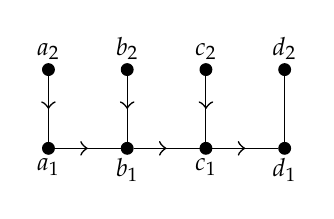
\begin{tikzpicture}[decoration={
        markings,
        mark=at position 0.5 with {\arrow[scale=1.5]{>}}}
      ]
      \foreach \x/\j in {a/0,b/1,c/2,d/3}{
        \foreach \i in {1,2}{
          \node[classic] (\x\i) at (\j,\i) {};
        }
        \node[below] at (\x1) {\small $\x_{1}$};
        \node[above] at (\x2) {\small $\x_{2}$};
      }
      
      \draw[postaction={decorate}] (a2) -- (a1);
      \draw[postaction={decorate}] (b2) -- (b1);
      \draw[postaction={decorate}] (c2) -- (c1);
      \draw (d1) -- (d2);
      
      \draw[postaction={decorate}] (a1) -- (b1);
      \draw[postaction={decorate}] (b1) -- (c1);
      \draw[postaction={decorate}] (c1) -- (d1);          
    \end{tikzpicture}
    \caption{A valid orientation of $C_i$. The edge $a_1a_2$ is negative, $b_1b_2$ and
        $c_1c_2$ are negative, and $d_1d_2$ can either be positive or negative.}
      \label{fig:variable_gadget}
    \end{figure}
  \end{poc}

  \paragraph{Equivalence of the instances.}
  We are now ready to prove that $\phi$ admits a valuation such that each
  clause contains both variables set to
  true and false if and only if
  $G_\phi$ is a $k$-iterated shift graph. In fact for the reverse direction, we will show the stronger property that if
  $\phi$ is not a positive instance of $\MNAE$, then then $G_\phi$ is not even a shift graph.

  We start proving the reverse implication and consider a valid orientation $\orGphi$ of
  $G_\phi$. We now consider the following variable assignment: for each variable $x$, set $x$ to true if $w^{0}_x \to v^0_x$ in $\orGphi$ and
  to false otherwise. We show that with this variable assignment, each clause of $\phi$ contains both variables set to true and false.
  Let $i\in \{0,\ldots,m-1\}$ and assume that the $i$\textsuperscript{th} clause of $\phi$ is $x\lor y\lor z$. 
  Recall that the corresponding comb $C_i$ of length $3$ in $G_{\varphi}$ has jaw $a_ib_ic_id_i:=w_x^{8i}w_y^{8i+2}w_y^{8i+6}w_z^{8i}$, and let $e_1,e_2,e_3,e_4$ denote the teeth of $C_i$, such that $e_1$ is incident to $a_i$, $e_2$ to $b_i$, $e_3$ to $c_i$ and $e_4$ to $d_i$. 
%   As $8i+2=2(4i+1)$ and $8i+6=2(4i+3)$, \cref{cl:gadget_orientation} implies that $e_2$ is positive in $\orGphi$ if and only if $e_3$ is.
Note that \cref{cl:gadget_orientation} implies that $e_1, e_2, e_4$ are respectively positive in $\orGphi$ if and only if $x,y,z$ are respectively set to true. In particular, \cref{cl:clause_orientation} then implies that at least one teeth of $C_i$ is positive, and one is negative in $\orGphi$. It then implies that the variable assignment we defined satisfies the desired properties.
  
%   By construction and by \cref{cl:gadget_orientation}, each
%   of the edges $e_1, \ldots, e_4$ attached to the internal vertices of $C_i$ is
%   positive if and only if the corresponding variable is true. By
%   \cref{cl:clause_orientation}, the edges $e_1, \ldots, e_4$ cannot be all
%   positive or all negative because the orientation is valid. Hence
%   $i$\textsuperscript{th} clause contains a true and a false variable, which
%   concludes the proof.


  We now prove the direct implication and consider a variable assignment for which each clause of $\phi$ contains both variables set to true and false.
  For
  each variable $x$, let $\orMx$ denote the (unique) valid orientation of $M_x$ given by \cref{cl:gadget_orientation} such that
  $w^{0}_x \to v^{0}_x$ in $\orMx$ if $x$ is set to true, and such that $v^0_x\to w^0_x$ in $\orMx$ if $x$ is set to false.
  Then, for each $i\in \{0,\ldots,4m-1\}$, we consider for each copy $H^i_x$ of the four-sun the (unique) valid orientation $\orHxi$ given by \cref{cl:sun_orientation}, such that in  $\orMx\cup\orHxi$, the vertex $t^{2i}_x$ has both in- and out-degrees equal to two. We let $\orLx$ denote the orientation obtained after orienting this way $M_x$ and all subgraphs $H_x^i$ of $L_x$. See   \cref{fig:oriented_variable}.

  
  
  
%   With a slight
%   abuse of notation, we will name the directed graph arising from the
%   progressive orientations of our gadgets with the same naming conventions.
%   For
%   each variable $x$, choose the unique valid orientation of $M_x$ such that
%   $w^{0}_x \to v^{0}_x$ if $x$ is true (by \cref{cl:gadget_orientation} there
%   exists only one such orientation). Then orient each copy of the four-sun such
%   that each $t^{2i}_x$ has in and out-degree equal to two (by
%   \cref{cl:sun_orientation}, there exists a unique such orientation for each
%   $(x,i)$). The orientation of each variable gadget $L_x$ is drawn on
%   \cref{fig:oriented_variable}.

    \begin{figure}[h!]
    \centering
    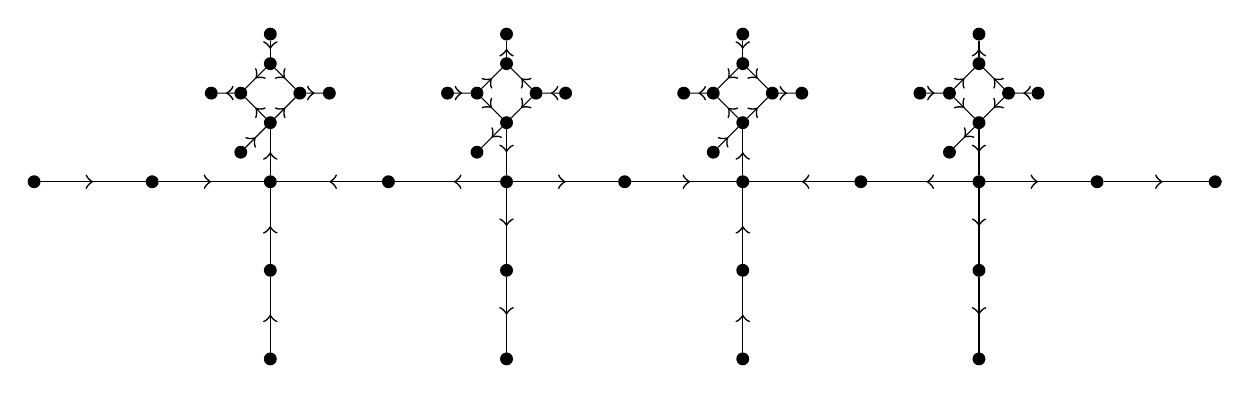
\begin{tikzpicture}[scale = 1.5,decoration={
        markings,
        mark=at position 0.5 with {\arrow[scale=1.5]{>}}}
      ]
      \foreach \i in {0,2}{
        \begin{scope}[shift={(2*\i,0)}]
          \node[classic] (a\i) at (0,0) {};
          
          \node[classic] (e\i1) at (0,-.75) {};
          \node[classic] (e\i2) at (0,-1.5) {};

          \node[classic] (H\i11) at (0,.5) {};
          \node[classic] (H\i12) at (-.25,.25) {};
          \node[classic] (H\i21) at (.25,.75) {};
          \node[classic] (H\i22) at (.5,.75) {};
          \node[classic] (H\i31) at (0,1) {};
          \node[classic] (H\i32) at (0,1.25) {};
          \node[classic] (H\i41) at (-.25,.75) {};
          \node[classic] (H\i42) at (-.5,.75) {};
          \draw[postaction={decorate}] (H\i11) to (H\i21);
          \draw[postaction={decorate}] (H\i11) to (H\i41);
          \draw[postaction={decorate}] (H\i31) to (H\i21);
          \draw[postaction={decorate}] (H\i31) to (H\i41);
          \draw[postaction={decorate}] (e\i1) to (a\i);
          \draw[postaction={decorate}] (a\i) to (H\i11);
          \draw[postaction={decorate}] (e\i2) to (e\i1);
          \foreach \j in {1,3}{
            \draw[postaction={decorate}] (H\i\j2) to (H\i\j1);
          }
          \foreach \j in {2,4}{
            \draw[postaction={decorate}] (H\i\j1) to (H\i\j2);
          }
        \end{scope}                
      }

      \foreach \i in {1,3}{
        \begin{scope}[shift={(2*\i,0)}]
          \node[classic] (a\i) at (0,0) {};
          
          \node[classic] (e\i1) at (0,-.75) {};
          \node[classic] (e\i2) at (0,-1.5) {};

          \node[classic] (H\i11) at (0,.5) {};
          \node[classic] (H\i12) at (-.25,.25) {};
          \node[classic] (H\i21) at (.25,.75) {};
          \node[classic] (H\i22) at (.5,.75) {};
          \node[classic] (H\i31) at (0,1) {};
          \node[classic] (H\i32) at (0,1.25) {};
          \node[classic] (H\i41) at (-.25,.75) {};
          \node[classic] (H\i42) at (-.5,.75) {};
          \draw[postaction={decorate}] (H\i21) to (H\i11);
          \draw[postaction={decorate}] (H\i21) to (H\i31);
          \draw[postaction={decorate}] (H\i41) to (H\i11);
          \draw[postaction={decorate}] (H\i41) to (H\i31);
          \draw[postaction={decorate}] (H\i11) to (a\i);
          \draw[postaction={decorate}] (a\i) to (e\i1);
          \draw[postaction={decorate}] (e\i1) to (e\i2);
          \foreach \j in {2,4}{
            \draw[postaction={decorate}] (H\i\j2) to (H\i\j1);
          }
          \foreach \j in {1,3}{
            \draw[postaction={decorate}] (H\i\j1) to (H\i\j2);
          }
          
        \end{scope}        
        
      }


      \node[classic] (a) at (-2,0) {};
      \node[classic] (b) at (-1,0) {};
      \node[classic] (a4) at (8,0) {};

      \draw[postaction={decorate}] (a) to (b);
      \draw[postaction={decorate}] (b)-- (a0);

      \foreach \i in {1,3}{
        \node[classic] (b\i) at (2*\i+1,0) {};
        \pgfmathsetmacro{\j}{\i+1}
        \draw[postaction={decorate}] (a\i) to (b\i);
        \draw[postaction={decorate}] (b\i)to (a\j);
      }
      \foreach \i in {0,2}{
        \node[classic] (b\i) at (2*\i+1,0) {};
        \pgfmathsetmacro{\j}{\i+1}
        \draw[postaction={decorate}] (a\j) to (b\i);
        \draw[postaction={decorate}] (b\i)to (a\i);
      }
      
       \end{tikzpicture}  
    \caption{The orientation of $L_x$ when $x$ is true (for the false variables,
    the orientation is reversed)}
    \label{fig:oriented_variable}    
  \end{figure}
  
  In order to obtain an orientation of $G_{\phi}$, 
  the only edges that remain to be oriented are the edges forming the jaw of
  each clause gadget. For each $i\in \{0,\ldots,m-1\}$, consider the comb $C_i$ corresponding to the
  $i$\textsuperscript{th} clause $x\lor y\lor z$ of $\phi$, and denote with $e_1,\ldots, e_4$ its teeth, again with respect to the order in which they attach to the jaw. 
  As $\orMy$ is a valid orientation of $M_y$, and as $8i+2= 2(4i+1)$ and $8i+6=2(4i+3)$,
  by
  \cref{cl:gadget_orientation}, $e_2$ and $e_3$ are either both negative or both
  positive. Moreover, observe that by definition of the orientations $\orMx, \orMy, \orMz$, \cref{cl:gadget_orientation} implies that $e_1,e_2,e_4$ are respectively positive if and only if $x,y,z$ are respectively set to true.
  Since the clause $x\lor y\lor z$ contains both variables set to true and false, we can apply
  \cref{cl:clause_orientation} to extend our orientation to a valid orientation $\orCi$ of $C_i$, in which the jaw is a directed path. Fixing such an orientation of each $C_i$, we now obtain an orientation $\orGphi$ of $G_{\phi}$, whose restriction to each subgraph of the form $L_x$ or $C_i$ is valid.
  
  \ugo{Do you want to keep the next paragraph? I do not think that it is useful.}
  In order to prove that $\orGphi$ is a valid orientation,
  we only need to
  check the first condition of \cref{lem:forbidden_config} at the junctions
  between the clause and the variable gadgets, and the orientation of the cycles
  using these junctions. Note that any such cycle must pass by some $u^{2i}_x$,
  at which it alternates. Finally, as each $u^{2i}_xv^{2i}_xw^{2i}_x$ forms a
  non-alternating path, the first condition of \cref{lem:forbidden_config} is
  satisfied and the orientation of $G_\phi$ is that of an acyclic line
  digraph. In other words, $G_\phi$ is a shift graph. This concludes the proof
  for shift graphs, but not for iterated shift graphs.

  
  
  To prove that $G_\phi$ is a $k$-iterated shift graph, we now construct an oriented
  acyclic graph $\orGphip$ such that $\orGphi$ is an induced subdigraph of
  $L^k(\orGphip)$. For each variable $x$, by \cref{lem:shift_tree}, there exists
  an acyclic oriented graph $\orMxp$ with a convex $k$-shift embedding $\psi_x$ of $\orMx$ in $\orMxp$.
  Similarly, for each clause comb $C_i$, there exists an acyclic oriented graph
  graph $\orCip$ with a convex $k$-shift embedding $\psi_i$ of $\orCi$ in
  $\orCip$. Denote $\psi$ the union of all these $k$-shift embedding. \ugo{What do you mean by union? I think that you need to define the image of $\psi$ properly, I do not understand.}
 
  
  
  
  
  
  
  
  
  
  
  
  
  
%   For each variable $x$, by \cref{lem:shift_tree}, there exists
%   a graph $M'_x$ with a convex $k$-shift embedding $\psi_x$ of $M_x$ in $M'_x$.
%   By \cref{lem:shift_tree}, for each clause comb $C_i$, there exists a
%   graph $C'_i$ with a convex $k$-shift embedding $\psi_i$ of $C_i$ in
%   $C'_i$. Denote $\psi$ the union of these $k$-shift embedding.

  First, we note that $(\psi(N(v^{2i}_x)))_{i,x}$ forms a collection of pairwise
  disjoint $k+2$-paths because any distinct $v^{2i}_x$ and $v^{2j}_y$ are
  either in different component of the support of $L_x$, or connected by a
  unique path $P$ containing a directed subpath of length $k+2$ between
  $v^{2i}_x$ and $u^{2i}_x$. As result, $\psi(N(v^{2i}_x))$ and $\psi(u^{2i}_x)$
  are vertex disjoint and since $\psi$ is convex, so are the extremities of $P$:
  $\psi(N(v^{2i}_x))$ and $\psi(N(v^{2j}_y))$. By iteratively applying
  \cref{lem:gluing} to identify the leaves of the gadgets $N_i$ to the gadget
  variables along the concerned vertices $v^{4i+2c}_x$ for some $c$, the images
  of the vertices to be indentified remain disjoint. At the end of
  this identification process, we have a $k$-shift embedding of $G_\phi$ minus
  the 4-suns.

  Finally, we identify each $\psi(t^{4i}_x)$ with the path of length $k$
  starting in the vertex $t$ of the graph $F$ drawn on \cref{fig:sun_root}. It
  is straightforward to check that the $k$-line digraph of the graph drawn on
  \cref{fig:sun_root} is the 4-sun and the resulting graph $G'_\phi$ is such
  that $G_\phi$ is an induced subgraph of $G'_\phi$.
  \begin{figure}[h!]
    \centering
    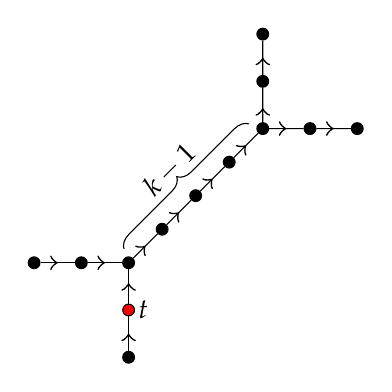
\begin{tikzpicture}[scale = .6,decoration={
        markings,
        mark=at position 0.5 with {\arrow[scale=1.5]{>}}}]
          
      \node[classic] (a1) at (-2,0) {};
      \node[classic] (a2) at (-1,0) {};
      \node[classic] (a3) at (0,0) {};
     
      \node[classic] (b1) at (0,-2) {};
      \node[classic, fill=red] (b2) at (0,-1) {};
      \node[right=0cm] at (b2) {$t$};
  
      \coordinate (b3) at (a3);

      \foreach \i in {1,...,3}{
        \node[classic] (v\i) at (0.71*\i,0.71*\i) {};
      }

      \begin{scope}[shift={(2.84,2.84)}]
        \node[classic] (c1) at (2,0) {};
        \node[classic] (c2) at (1,0) {};
        \node[classic] (c3) at (0,0) {};
        
        \node[classic] (d1) at (0,2) {};
        \node[classic] (d2) at (0,1) {};
        \coordinate (d3) at (c3);
      \end{scope}

      \foreach \u in {a,b}{
        \draw[postaction={decorate}] (\u1) to (\u2);
        \draw[postaction={decorate}] (\u2) to (\u3);
      }
      \foreach \u in {c,d}{
        \draw[postaction={decorate}] (\u3) to (\u2);
        \draw[postaction={decorate}] (\u2) to (\u1);
      }

      \draw[postaction={decorate}] (a3) to (v1);
      \draw[postaction={decorate}] (v1) to (v2);
      \draw[postaction={decorate}] (v2) to (v3);
      \draw[postaction={decorate}] (v3) to (c3);

      \draw [decorate,decoration={brace,amplitude=5pt,mirror,raise=1ex}] (c3) -- (a3) node[midway,xshift=-2ex,yshift=2ex,rotate=45]{$k-1$};
    \end{tikzpicture}  
    \caption{A graph $F$ whose $k$-line digraph is the $4$-sun.}
    \label{fig:sun_root}    
  \end{figure}
\end{proof}



\section{Attempt for iterated shift}


It would be great if ``iterated shift'' would be equivalent to ``shift
of high odd girth''.  Here is an attempt in the infinite odd girth
case (that is for bipartite graphs).

\begin{theorem}
  If $G$ is a bipartite acyclic shift graph, then there exits a bipartite
  acyclic shift graph $H$ such that $G$ is an induced subgraph of $L(H)$.
\end{theorem}

\begin{proof}
   Since $G$ is an acyclic shift graph, consider an acyclic graph $R$
   such that $G = L(R)$.  Assume furthermore that every sink and every
   source and every sink of $R$ has degree~1 (by some lemma ??).

   We claim that $R$ is bipartite.  
\end{proof}


\section*{Acknowledgements}
The research was initiated during a one-week research visit by Nicolas Trotignon
at Jagiellonian University in January 2025, supported by the grant FILL.

\nocite{*}
\bibliographystyle{abbrv}
\bibliography{references}

% \appendix
% \section{Code use for the computer check of \cref{thm:3col}}\label{sec:computer_check}
% To check that all 3-arc-colourings of $H$ colour the two arcs entering $x$ with
% different colours, we compute the number of 3-colourings of $L(H)$ and the
% number of 3-colourings of $G$, where $G$ is obtained from $L(H)$ by
% adding an edge betwenn the vertices correspoding to arcs entering $x$ in
% $H$. The following code shows that these numbers are equal, so all 3-colourings
% of $L(H)$ are 3-colourings of $G$, which implies the desired result.
% \begin{lstlisting}[language=Python]
% from sage.graphs.graph_coloring import chromatic_number, number_of_n_colorings

% # Constructing L(H)
% vertices = [(i,j) for i in range(7) for j in range(i+1,7) if j-i <= 4]
% for i in [3,4]:
%     vertices.append((i,7))
% for i in [5,6]:
%     vertices.append((i,9))  # the vertex x of H is labelled 9 here
% for i in [4,5,6]:
%     vertices.append((i,8))
% d =dict()
% for u in vertices: 
%     L = [v for v in vertices if (v[1] == u[0] or v[0] == u[1])] 
%     d[u] = L
% LH = Graph(d)

% # Computing the number of 3-colourings
% print("L(H) has " + str(number_of_n_colorings(LH,3)) + " proper 3-colourings")
% LH.add_edge((6,9),(5,9)) # LH is now the graph G
% print("G has " + str(number_of_n_colorings(LH,3)) + " proper 3-colourings")
% \end{lstlisting}

\end{document}

